% !TeX encoding = UTF-8
% !TeX spellcheck = en_US
\documentclass[a4paper,
	DIV=12,
	BCOR=1cm,
	twoside,
	toc=listofnumbered,
	bibliography=totocnumbered,
	numbers=noenddot,
	abstract=on
	]{scrreprt}
	\usepackage[utf8]{inputenc} % Sonderzeichen
	\usepackage{fancyhdr} % Kopf-, Fußzeilen
	\usepackage{graphicx} % Bilder	
	\usepackage[bookmarksopen,
				bookmarksopenlevel=0,
				pdfborder={0 0 0}]{hyperref} % Hyperlinks
	\usepackage{amsmath} % Mathe, lädt amsmath gleich mit
	\usepackage{amssymb} % Mathesymbole
	\usepackage{paralist} % Nummerierungen a) etc. von Umgebungen
	\usepackage{todonotes}
	\usepackage{setspace}
	\usepackage{float}
	\usepackage[lofdepth,lotdepth]{subfig}

	\usepackage{thmbox}
	\newtheorem[style=M, bodystyle={\noindent}]{theorem}{Theorem}
	\newtheorem[style=M, bodystyle={\noindent}]{definition}[theorem]{Definition}

	\usepackage{etoolbox}
	\BeforeBeginEnvironment{theorem}{\vskip 0.3cm}
	\BeforeBeginEnvironment{definition}{\vskip 0.3cm}

	\usepackage{changepage}

	% Import title etc. constants
	% !TeX spellcheck = en_US
\def\Author{Patrick Robrecht}
\def\ThesisType{Master's Thesis}
\def\Title{Incremental Unidirectional Model Transformation via Graph Transformation with eMoflon::IBeX}
\def\Keywords{graph transformation, graph transformation tool, eMoflon, model transformation, unidirectional model transformation, model modification}

\def\Supervisor{Jun.-Prof. Dr. Anthony Anjorin}
\def\SecondExaminer{Prof. Dr. Gregor Engels}
\def\DateOfProposalSubmission{March 8, 2018}
\def\DateOfThesisSubmission{July 12, 2018}

\def\ResearchGroup{Database and Information Systems}
\def\Address{Fürstenallee 11, 33102 Paderborn}

% own commands
\newcommand{\eg}{e.\,g. }
\newcommand{\ie}{i.\,e. }
\newcommand{\create}{{\color[rgb]{0,0.5,0} \texttt{++}}}
\newcommand{\delete}{{\color[rgb]{1,0,0} \texttt{--}}}

% common includes
\usepackage{tikz}
\usetikzlibrary{
	arrows,
	calc,
	positioning
}

% (class diagrams)
\usepackage{../../master-thesis-gt-tool/common/tikz-uml}
\tikzset{
	class/.style = {
		inner sep = 0
	}
}
\newcommand{\methodSep}{\\[-4px]}

% tables
\renewcommand{\arraystretch}{1.5}
\usepackage{longtable} % allows to use footnotes in table
\usepackage{booktabs}
\usepackage{pifont}
\newcommand{\yes}{{\color{green}$\checkmark$}}
\newcommand{\no}{{\color{red}\text{\ding{55}}}}

% listings
\definecolor{commentcolor}{rgb}{0,0.4,0.2}
\definecolor{keywordcolor}{rgb}{0.50,0.00,0.33}

\usepackage{listings}
\lstset{
	aboveskip = 15pt,
	basicstyle = \small\ttfamily,
	breaklines = true,
	captionpos = b,
	commentstyle = \color{commentcolor},
	emphstyle = \bfseries,
	numbers = left,
	numbersep = 10pt,
	numberstyle = \scriptsize \color{gray},
	keywordstyle = \color{keywordcolor},
	language = Java,
	tabsize = 4,
	xleftmargin = 20pt,
	frame = lrtb,
	framexbottommargin = 5pt,
	framexleftmargin = 20pt,
	framexrightmargin = 5pt,
	framextopmargin = 5pt
}


	\hypersetup{
		pdftitle = {\Title},
		pdfsubject = {\ThesisType},
		pdfauthor = {\Author},
		pdfkeywords = {\Keywords},
	}

	\setcounter{tocdepth}{10} % all levels into table of contents.
	\setcounter{secnumdepth}{10} % numbering even for level 4+

% Title Settings
	\title{Master Thesis: \Title}
	\author{\Author}
	\date{\DateOfThesisSubmission}


\begin{document}
	\addtolength{\oddsidemargin}{0.75cm}
	\begin{titlepage}
		\begin{center}
			\begin{minipage}{13.5cm}		
				\includegraphics[height = 2.4cm]{../common/figures/university-logo-en} \\[3pt]
				\textsf{
					\hspace*{2.2cm} Faculty for Computer Science, Electrical Engineering and Mathematics \\
					\hspace*{2.2cm} Department of Computer Science \\
					\hspace*{2.2cm} \ResearchGroup \\
					\hspace*{2.2cm} \Address
				}
			\end{minipage}\\[60pt]

			{\Huge\bfseries
				Incremental Unidirectional \\
				Model Transformation \\
				via Graph Transformation \\[5pt]
				with eMoflon::IBeX} \\[30pt]

			{\LARGE \ThesisType} \\[15pt]
			in Partial Fulfillment of the Requirements for the\\
			Degree of \\[15pt]
			{\Large Master of Science} \\[30pt]

			by \\[5pt]

			{\scshape\large \Author} \\[30pt]

			submitted to \\[5pt]

			{\scshape\large \Supervisor} \\[5pt]

			and \\[5pt]

			{\scshape\large \SecondExaminer} \\[40pt]

			{Paderborn, \DateOfThesisSubmission}
		\end{center}
	\end{titlepage}
	\addtolength{\oddsidemargin}{-0.75cm}

	% header and footer
	\newcommand{\fancy}{
		\fancyhf{}
		\renewcommand{\headrulewidth}{0.0pt}
		\fancyfoot[C]{}
		\fancyfoot[LO,RE]{\scriptsize \Title}
		\fancyfoot[LE,RO]{\small \thepage}
		\renewcommand{\footrulewidth}{0.5pt}
	}
	\pagestyle{fancy}
	\fancy
	\fancypagestyle{plain}{\fancy}


\newpage
	\thispagestyle{empty}
	~\ \\[430pt]

	\textcopyright~2018 \Author
	\ \\

	Master's Thesis by \Author

	Course of studies: Computer Science
	\ \\

	Supervisor: \Supervisor
	\ \\

	First examiner: \Supervisor

	Second examiner: \SecondExaminer
	\ \\

	Date of submission: \DateOfThesisSubmission


	% !TeX encoding = UTF-8
% !TeX spellcheck = en_US

\pdfbookmark[1]{Abstract}{abstract}
\begin{abstract}
	Model transformations are used to transform models into other models.
	They are fundamental for model-driven engineering (MDE) which raises the abstraction level from programming to domain-specific languages.
	As models can be suitably represented as graphs, graph transformation (GT) is a frequently used formalism to realize model transformations.
	The approach is based on a rule set defining which graph patterns can be replaced with other graph structures.

	This thesis presents eMoflon::IBeX-GT, a new interpreter-based graph transformation tool which supports model queries (\ie finding patterns in the graph) as well as rule applications modifying graph structures.
	An incremental pattern matcher is used to find matches in the host graph.
	The support for incrementality is important to solve tasks which require permanent observation of all matches efficiently.

	The graph transformation patterns and rules can be invoked from Java code via a typed API generated from the textual specification.
	Pattern refinement is a modularity concept to reduce duplications in pattern specifications.
	
	There are many GT tools, but to the best of the author's knowledge none of them supports incrementality in combination with model queries and rule applications on attributed typed graphs via a typed API.

	This thesis explores which tasks can be solved best via an incremental graph transformation tool and how the tool can be seamlessly integrated into Java code.
\end{abstract}



	\pdfbookmark[1]{Table of Contents}{toc}
	\tableofcontents


	\chapter*{Declaration of Authorship}
		I hereby declare that I prepared this thesis entirely on my own and have not used outside sources without declaration in the text.
		Any concepts or quotations applicable to these sources are clearly attributed to them.
		This thesis has not been submitted in the same or substantially similar version, not even in part, to any other authority for grading and has not been published elsewhere.\\[27pt]

		Paderborn, \DateOfThesisSubmission \\[20pt]

		\Author

	\newpage

	% !TeX encoding = UTF-8
% !TeX spellcheck = en_US

\section{Introduction}

\subsection{Running Example}
	\begin{frame}
		\frametitle{Introduction}
		\framesubtitle{Running Example: She Remembered Caterpillars}
		\begin{center}
			\vspace{-4mm}
			\includegraphics[height=.82\textheight]{../common/figures/she-remembered-caterpillars-game}
		\end{center}
	\end{frame}
	\begin{frame}
		\frametitle{Introduction}
		\framesubtitle{Running Example: She Remembered Caterpillars Ecore Meta-Model}
		\begin{center}
			\includegraphics[width=\linewidth]{../common/figures/she-remembered-caterpillars-class-diagram}
		\end{center}
	\end{frame}

\subsection{Unidirectional Graph Transformation}
	\begin{frame}
		\frametitle{Introduction}
		\framesubtitle{Unidirectional Graph Transformation: An Example Rule}
		\begin{center}
			\includegraphics[height=.75\textheight]{../common/figures/rule-moveCharacterToNeighboringPlatform}
		\end{center}
	\end{frame}

\subsection{Main Requirements}
	\begin{frame}
		\frametitle{Introduction}
		\framesubtitle{Main Requirements for a Graph Transformation Tool}
		\begin{enumerate}
			\item Incremental interpreter
				\only<1>{
					\begin{itemize}
						\item Idea: store set of matches of a rule and maintain it whenever the model changes
						\item Pattern matching more efficient 
					\end{itemize}
				}
			\item Integration with a TGG tool
				\only<2>{
					\begin{itemize}
						\item Advantages for developers: shared code, reduce maintenance effort. 
						\item Advantages for users: same meta-models and similar rule syntax for TGGs and GTs
					\end{itemize}
				}
			\item Java API
				\only<3>{
					\begin{itemize}
						\item Easy to use
						\item Type safe
					\end{itemize}
				}
			\item Expressive GT language
				\only<4>{
					\begin{itemize}
						\item Rule refinement
						\item Application conditions
						\item Attribute manipulation
					\end{itemize}
				}
			\item Textual syntax and generated visualization \\
				\only<5>{
					\begin{itemize}
						\item Text for easy editor support and versioning
						\item Visualization for users
					\end{itemize}
				}
		\end{enumerate}
	\end{frame}

\subsection{Comparison of Existing Tools with respect to the Requirements}
	\begin{frame}
		\frametitle{Introduction}
		\framesubtitle{Comparison of Existing Graph Transformation Tools with respect to the Requirements}
		\begin{block}{Comparison Results}
			\begin{itemize}
				\item VIATRA only incremental tool, but no support for GT.
				\item No GT tool supports incrementality.
				\item Most GT tools offer only limited support for application conditions and attribute manipulation.
				\item No GT tool supports rule refinement.
			\end{itemize}
		\end{block}
	\end{frame}

	% !TeX encoding = UTF-8
% !TeX spellcheck = en_US

\chapter{Fundamentals of Graph Transformations}
\label{fundamentals}
This chapter introduces the formal definitions for graph transformations based on category theory.
The definitions are based on Ehrig et al. \cite[pp. 21-47 and pp. 65-71]{FundamentalsOfAlgebraicGT} in a slightly different notation used in the lecture ``Fundamentals of Model-Driven Engineering'' by Anthony Anjorin.

\newcommand{\st}{.~}
\newcommand{\then}{\textbf{\,;\,}}
\newcommand{\gap}{\medskip \noindent}

\newcommand{\Graphs}{\textbf{Graphs}}
\newcommand{\TGraphs}{\textbf{TGraphs}}

% !TeX encoding = UTF-8
% !TeX spellcheck = en_US

\tikzset{
	defpicture/.style = {
		auto,
		node distance = 2cm,
		arrow/.style = {
			draw,
			->,
			shorten >=2pt,
		}
	},
	defnode/.style = {
		circle,
		draw = black
	},
	def1/.style = {
		text = red
	},
	def1-arrow/.style = {
		draw = red
	},
	def2/.style = {
		text = blue
	},
	def2-arrow/.style = {
		draw = blue
	}
}

% !TeX encoding = UTF-8
% !TeX spellcheck = en_US

\tikzset{
	tgraph/.style = {
		node distance = 0.5cm
	},
	tnode/.style = {
		fill = blue!10,
		inner sep = 3pt
	},
	tedge/.style = {
		draw = blue!50,
		thick,
		->
	},
	dlabel/.style = {
		inner sep = 1pt
	},
	dnode/.style = {
		draw = orange,
		thick,
		inner sep = 8pt
	},
	dedge/.style = {
		draw = orange,
		thick,
		->
	}
}


\section{Typed Graphs}
\label{fundamentals-typed-graphs}
Our models are attributed typed graphs.
Typed graphs are formally introduced in the following, while attributes are not formalized in this thesis.
The interested reader is referred to \cite{AttributedGraphTransformationViaRuleSchemata} or \cite{ComplexAttributeManipulationInTGGs} for a formalization of attributed graphs.

\begin{definition}[Category]
	\label{def:category}%
	A category $\mathbf{C} = (Ob, Arr, \then , id)$ consists of:
	\begin{itemize}
		\item a class $Ob$ of \emph{objects},
		\item for each pair of objects $A, B \in Ob$, a class $Arr_{(A, B)}$ of \emph{arrows},\\ where $f \in Arr_{(A,B)}$ is denoted by $f: A \rightarrow B$,
		\item for all objects $A, B, C \in Ob$,  a binary operation (for composing arrows):\\ 
		$\then: Arr_{(A,B)} \times Arr_{(B,C)} \rightarrow Arr_{(A,C)}$,
		\item for each object $A \in Ob$, an identity arrow $id_A: A \rightarrow A$,
	\end{itemize}
	such that the following conditions hold:
	\begin{itemize}
		\item Associativity.\\ $\forall A,B,C,D \in Ob\st \forall f: A \rightarrow B, g: B \rightarrow C, h: C \rightarrow D\st f \then (g \then h) = (f \then g) \then h$.
		\item Identity.\\ $\forall A, B \in Ob\st \forall f: A \rightarrow B\st (id_A \then f = f) \wedge (f \then id_B = f)$.
	\end{itemize}
\end{definition}

\noindent
In general, a category is a mathematical structure which has objects and morphisms.
A monomorphic arrow corresponds to an injective function.

\begin{definition}[Monomorphism]
	\label{def:monomorphism}%
	Let $\mathbf{C} = (Ob, Arr, \then , id)$ be a category.

	\gap
	An arrow \textcolor{red}{$f : X \rightarrow Y$} is monomorphic, iff 
	\[
		\forall\, g: Z \rightarrow X~ \forall\, h: Z \rightarrow X~ [(h;f = g;f) \Rightarrow (g = h)].
	\]
\end{definition}

\begin{figure}[h!]
	\centering
	\begin{tikzpicture}[defpicture]
	\node (Z) {$Z$};
	\node[def1, right of = Z] (X) {$X$};
	\node[def1, right of = X] (Y) {$Y$};

	\begin{scope}[every path/.style = arrow]
		\path (Z.20) to[bend left] node[above] {g} (X.160);
		\path (Z.340) to[bend right] node[below] {h} (X.200);
		\path[def1-arrow] (X) to node[def1] {f} (Y);
	\end{scope}
\end{tikzpicture}

	\caption{Monomorphism}
	\label{fig:monomorphism}
\end{figure}

\begin{definition}[Graphs and Graph Morphisms]
	\label{def:graphs}%
	A \emph{graph} \textcolor{red}{$G = (V, E, src, trg)$} consists of a set \textcolor{red}{$V$} of nodes (vertices), a set \textcolor{red}{$E$} of edges, and two functions \textcolor{red}{$src, trg: E \rightarrow V$} that assign each edge a source node and a target node, respectively.

	\gap
	Given graphs $G = (V, E,src,trg)$ and $G' = (V', E', src', trg')$, a \emph{graph morphism} \textcolor{blue}{$f: G \rightarrow G'$} consists of two functions
	\textcolor{blue}{$f_V: V \rightarrow V'$}
	and \textcolor{blue}{$f_E: E \rightarrow E'$}
	such that $src \then f_V = f_E \then src'$ and $trg \then f_V  = f_E \then trg'$.

	\gap
	$\Graphs = (Ob_{Graphs}, Arr_{Graphs}, \then_{Graphs}, id_{Graphs})$ consists of:
	\begin{itemize}
		\item graphs $Ob_{Graphs}$,
		\item graph morphisms $Arr_{Graphs}$,
		\item for $G, G', G'' \in Ob_{Graphs}$, $f =  G \rightarrow G'$, $g = G' \rightarrow G'' \in Arr_{Graphs}$, 
		$\then_{Graphs} (f,g) $ is defined as $f \then_{Graphs}~g := (f_V \then g_V, f_E \then g_E)$, 
		\item for $G = (V, E, src,trg) \in Ob_{Graphs}$,
		$id_G: G \rightarrow G$ is defined as $id_G := (id_V, id_E)$.
	\end{itemize}
\end{definition}

\begin{figure}[h!]
	\centering
	\begin{tikzpicture}[defpicture]
	\node[def1] (E) {$E$};
	\node[below of = E] (E') {$E'$};
	\node[def1, right of = E] (V) {$V$};
	\node[below of = V] (V') {$V'$};
	\node[def1, right = 1.5cm of V] (G) {$G = (E, V, src, trg)$};
	\node[below of = G] (G') {$G' = (E', V', src', trg')$};

	\begin{scope}[every path/.style = arrow]
		\path[def1-arrow] (E.20) to[bend left] node[def1, above] {src} (V.160);
		\path[def1-arrow] (E.340) to[bend right] node[def1, below] {trg} (V.200);

		\path[def2-arrow] (E) to node[def2, left] {$f_E$} (E');
		\path[def2-arrow] (V) to node[def2] {$f_V$} (V');

		\path (E'.20) to[bend left] node[above] {src'} (V'.160);
		\path (E'.340) to[bend right] node[below] {trg'} (V'.200);

		\path[def2-arrow] (G) to node[def2] {$f = (f_V, f_E)$} (G');
	\end{scope}
\end{tikzpicture}

	\caption{Graph Morphism}
	\label{fig:graph-morphism}
\end{figure}

\begin{definition}[Typed Graphs and Typed Graph Morphisms]
	\label{def:typed-graphs}%
	A \emph{type graph} is a distinguished graph $TG = (V_{TG}, E_{TG}, src_{TG}, trg_{TG})$.

	\gap
	A \emph{typed graph} is a pair $\hat{G} = (G, type)$ of a graph $G$ together with a graph morphism \textcolor{red}{$type: G \rightarrow TG$}.

	\gap
	Given typed graphs $\hat{G} = (G, type)$ and $\hat{G}' = (G', type')$, a \emph{typed graph morphism} $f: \hat{G} \rightarrow \hat{G}'$ is a graph morphism \textcolor{blue}{$f: G \rightarrow G'$} such that $f \then type' = type$.

	\gap
	$\TGraphs = (Ob_{TGraphs}, Arr_{TGraphs}, \then_{TGraphs}, id_{TGraphs})$ consists of:
	\begin{itemize}
		\item typed graphs $Ob_{TGraphs}$,
		\item typed graph morphisms $Arr_{TGraphs}$,
		\item $\then_{TGraphs} := \then_{Graphs}$,
		\item $id_{TGraphs} := id_{Graphs}$.
	\end{itemize}
\end{definition}

\noindent
Note that $\Graphs$ and $\TGraphs$ are categories according to Definition~\ref{def:category}.

\begin{figure}[h!]
	\centering
	\begin{tikzpicture}[defpicture]
	\node (TG) {$TG$};
	\node[def1, below of = TG] (G) {$G$};
	\node[right of = G] (G') {$G'$};

	\begin{scope}[every path/.style = arrow]
		\path[def1-arrow] (G) to node[def1, left] {type} (TG);
		\path[def2-arrow] (G) to node[def2, below] {f} (G');
		\path (G') to node[right] {type'} (TG);
	\end{scope}
\end{tikzpicture}

	\caption{Typed Graph Morphism}
	\label{fig:typed-graph}
\end{figure}

\noindent
Figure~\ref{fig:example-type-graph} shows the type graph for the She Remembered Caterpillars meta-model introduced in Section~\ref{running-example}.
For clarity only the types used in the following examples are included.
A typed graph conforming to this type graph is shown in Figure~\ref{fig:example-typed-graph-instance}.
Each node is denoted by its name and its type, separated by a colon.
The edge labels are omitted in the graphs as they are comprehensible without ambiguity based on the types of their source and target node.

\begin{figure}[h!]
	\centering
	% !TeX encoding = UTF-8
% !TeX spellcheck = en_US

\begin{tikzpicture}
	\node[tnode] (game) {Game};
	\node[tnode, below = of game, xshift = -2cm] (character) {Character};
	\node[tnode, below = of game, xshift = 2cm] (platform) {Platform};

	\draw[tedge]
		(game)
		-- node[left, xshift = -0.2cm, yshift = 0.2cm] {characters}
		(character);
	\draw[tedge]
		(game)
		-- node[right, xshift = 0.2cm, yshift = 0.2cm] {platforms}
		(platform);
	\draw[tedge]
		(character)
		-- node[below] {standsOn}
		(platform);
	\draw[tedge]
		(platform.south)
		-- ++(0, -1)
		-- ++(1.25, 0)
		-- ++(0, 1.25)
		-- node[right, xshift = 0.3cm] {neighbors}
		(platform.east);
\end{tikzpicture}

	\caption{Type Graph for She Remembered Caterpillars (simplified)}
	\label{fig:example-type-graph}
\end{figure}

\begin{figure}[h!]
	\centering
	% !TeX encoding = UTF-8
% !TeX spellcheck = en_US

\begin{tikzpicture}
	\node[tnode] (g) {g: Game};
	\node[tnode, below = of g] (p) {p: Platform};
	\node[tnode, left = of p] (c) {c: Character};
	\node[tnode, right = of p] (q) {q: Platform};

	\draw[tedge] (g.west) -- (c);
	\draw[tedge] (c) -- (p);
	\draw[tedge] (g) -- (p);
	\draw[tedge] (g.east) -- (q);
	\draw[tedge] (p) -- (q);
\end{tikzpicture}

	\caption{Typed Graph Instance}
	\label{fig:example-typed-graph-instance}
\end{figure}

\section{Rule Applications}
\label{fundamentals-rule-applications}
A set of rules defines which model modifications are allowed in the graph transformation system.
The semantics of rule applications is given by the following definitions.

\begin{definition}[Pushouts]
	\label{def:pushouts}%
	Let $\mathbf{C} = (Ob, Arr, \then, id)$ be a category.

	\gap
	Given arrows \textcolor{red}{$r \in Arr: L \rightarrow R$} and \textcolor{red}{$m \in Arr: L \rightarrow G$}, a \emph{pushout} $(G', r', m')$ over $r$ and $m$ is defined by
	a \emph{pushout object} \textcolor{blue}{$G' \in Ob$}, and
	morphisms \textcolor{blue}{$r': G \rightarrow G'$}, \textcolor{blue}{$m': R \rightarrow G'$},
	where
	\begin{enumerate}
		\item the ``pushout square'' (Figure~\ref{fig:pushout}) commutes, \ie $r \then m' = m \then r'$,
		\item and the following universal property is fulfilled:\\
		$\forall\, G'' \in Ob~ \forall\, r'': G \rightarrow G''~ \forall\, m'': R \rightarrow G''$\\
		$[(r \then m'' = m \then r'') \Rightarrow (\exists!\, x: G' \rightarrow G''\, [(m' \then x = m'') \wedge (r' \then x = r'')])]$.
	\end{enumerate}
	The category $\mathbf{C}$ is said to \emph{have pushouts} if the pushout $(G', r', m')$ always exists. 
\end{definition}

\begin{figure}[h!]
	\centering
	\begin{tikzpicture}[defpicture]
	\node (L) {$L$};
	\node[right of = L] (R) {$R$};
	\node[below of = L] (G) {$G$};
	\node[def2, right of = G] (G') {$G'$};
	\node[right of = G', yshift = -2cm] (G'') {$G''$};

	\begin{scope}[every path/.style = arrow]
		\path[def1-arrow] (L) to node[def1] {$r$} (R);
		\path[def1-arrow] (L) to node[def1, left] {$m$} (G);
		\path[def2-arrow] (R) to node[def2] {$m'$} (G');
		\path[def2-arrow] (G) to node[def2, below] {$r'$} (G');
	\end{scope}

	\begin{scope}[every path/.style = arrow, dashed]
		\path (R) to[bend left] node {$m''$} (G'');
		\path (G) to[bend right] node {$r''$} (G'');
		\path (G') to node {$x$} (G'');
	\end{scope}
\end{tikzpicture}

	\caption{Pushout Diagram}
	\label{fig:pushout}
\end{figure}

\begin{figure}[h!]
	\centering
	% !TeX encoding = UTF-8
% !TeX spellcheck = en_US

\begin{tikzpicture}[remember picture]
	\node[dnode] (L) {
    	\begin{tikzpicture}[tgraph]
    	    \node[dlabel] (label) {$\mathbf{L}$};
	    	\node[tnode, below = 0.2cm of label] (g) {g: Game};
	    	\node[tnode, below = of g] (p) {p: Platform};
	    	\draw[tedge] (g) -- (p);
    	\end{tikzpicture}
  	};

  	\node[dnode, right = 1.2cm of L] (R) {
    	\begin{tikzpicture}[tgraph]
    		\node[dlabel] (label) {$\mathbf{R}$};
			\node[tnode, below = 0.2cm of label] (c) {c: Character};
			\node[tnode, below = of c] (g) {g: Game};
			\node[tnode, below = of g] (p) {p: Platform};
			\draw[tedge] (c)
				-- ++(-1.5,0)
				-- ++(0,-2.13)
				-- (p);
			\draw[tedge] (g) -- (c);
			\draw[tedge] (g) -- (p);
		\end{tikzpicture}
   	};

	\node[dnode, below = 2cm of L] (G) {	  	
		\begin{tikzpicture}[tgraph]
			\node[dlabel] (label) {$\mathbf{G}$};
		   	\node[tnode, below = 0.2cm of label] (g) {g: Game};
		   	\node[tnode, below = of g] (p) {p: Platform};
		   	\node[tnode, below = of p] (q) {q: Platform};
		   	\draw[tedge] (g) -- (p);
		   	\draw[tedge] (g.east)
			   	-- ++(0.6,0)
			   	-- ++(0,-2.13)
			   	-- (q.east);
		   	\draw[tedge] (p) -- (q);
	   	\end{tikzpicture}
	};

	\node[dnode, below = 1cm of R] (G') {
    	\begin{tikzpicture}[tgraph]
       	    \node[dlabel] (label) {$\mathbf{G'}$};
			\node[tnode, below = 0.2cm of label] (c) {c: Character};
			\node[tnode, below = of c] (g) {g: Game};
			\node[tnode, below = of g] (p) {p: Platform};
			\node[tnode, below = of p] (q) {q: Platform};
			\draw[tedge] (c)
				-- ++(-1.5,0)
				-- ++(0,-2.13)
				-- (p);
			\draw[tedge] (g) -- (c);
			\draw[tedge] (g) -- (p);
			\draw[tedge] (g.east)
				-- ++(0.6,0)
				-- ++(0,-2.13)
				-- (q.east);
			\draw[tedge] (p) -- (q);
		\end{tikzpicture}
   	};

	\draw[dedge] (L) -- node[above] {$r$} (R);
	\draw[dedge] (L) -- node[left] {$m$} (G);
	\draw[dedge] (R) -- node[right] {$m'$} (G');
	\draw[dedge] (G) -- node[below] {$r'$} (G');
\end{tikzpicture}

	\caption{Application of the Monotonic Rule \texttt{createCharacter}}
	\label{fig:example-monotonic-rule-application}
\end{figure}

\noindent
An application of a monotonic rule $r: L \rightarrow R$ requires finding a match in the host graph $G$ (\ie a monomorphic arrow $m: L \rightarrow G$) 
and constructing the resulting host graph $G'$ by applying the changes (\ie constructing the monomorphic arrow $m': R \rightarrow G'$) such that the constraints above are fulfilled.
$m'$ is called \emph{co-match}.
The universal property ensures that no elements are glued unnecessarily, while the commutation in the pushout square rejects all results $G'$ that do not glue enough.

Figure~\ref{fig:example-monotonic-rule-application} illustrates the pushout construction for a rule \texttt{createCharacter} which creates a new character and connects the character to a platform and the game.

\begin{definition}[Graph Transformation Rules]
	\label{def:graph-transformation-rules}%
	A \emph{(typed) graph transformation rule} \textcolor{red}{$L \stackrel{l}{\hookleftarrow} K \stackrel{r}{\hookrightarrow} R$} is a pair of monomorphic arrows in the category of (\textbf{T})\textbf{Graphs} with common ``gluing graph'' $K$. 
\end{definition}

\noindent
Monotonic rules can only handle creation, but not deletion of elements.
That is why the formalism $L \stackrel{l}{\hookleftarrow} K \stackrel{r}{\hookrightarrow} R$ is introduced in Definition~\ref{def:graph-transformation-rules}:
$l: K \hookrightarrow L$ describes the deletion, $r: K \hookrightarrow R$ the creation of elements.
The elements in $L \setminus K$ are deleted by the rule, the elements in $R \setminus K$ are created.
All elements in K remain unchanged.

In the following chapters of this thesis, graph transformation rules which do not have deleted or created elements (\ie $L \setminus K = \emptyset = R \setminus K$) are referred to as \textit{graph transformation patterns}.

\begin{definition}[Double-Pushout Graph Transformation Rule Application]
	\label{def:dpo-rule-application}%
	Given a (typed) graph transformation rule \textcolor{red}{$p = L \stackrel{l}{\hookleftarrow} K \stackrel{r}{\hookrightarrow} R$}, a \emph{direct derivation} with $p$ at a monomorphism $m: L \hookrightarrow G$, denoted by $G\stackrel{p@m}{\Longrightarrow}\textcolor{blue}{G'}$ (or $G\stackrel{p}{\Rightarrow}G'$, or $G \Rightarrow G'$), is given by the double-pushout (DPO) diagram below, where $(1)$ and $(2)$ are pushouts in the category \textbf{(T)Graphs}. 
\end{definition}

\begin{figure}[h!]
	\centering
	\begin{tikzpicture}[defpicture]
	\node[def1] (L) {$L$};
	\node[def1, right of = L] (K) {$K$};
	\node[def1, right of = K] (R) {$R$};

	\node[below of = L] (G) {$G$};
	\node[right of = G] (D) {$D$};
	\node[def2, right of = D] (G') {$G'$};

	\node[xshift = 1cm, yshift = -1cm] (s1) {(1)};
	\node[xshift = 3cm, yshift = -1cm] (s2) {(2)};

	\begin{scope}[every path/.style = arrow]
		\path[def1-arrow] (K) to node[def1, above] {$l$} (L);
		\path[def1-arrow] (K) to node[def1, above] {$r$} (R);

		\path (L) to node[left] {$m$} (G);
		\path (K) to node {$d$} (D);
		\path (R) to node {$m'$} (G');

		\path (D) to node[below] {$l'$} (G);
		\path (D) to node[below] {$r'$} (G');
	\end{scope}
\end{tikzpicture}

	\caption{Double-Pushout Diagram}
	\label{fig:double-pushout}
\end{figure}

\begin{definition}[Applicability of Graph Transformation Rules]
	\label{def:rule-applicability}%
	A (typed) graph transformation rule \textcolor{red}{$p = L \stackrel{l}{\hookleftarrow} K \stackrel{r}{\hookrightarrow} R$} is applicable to a (typed) graph $G$ via the  match $m: L \hookrightarrow G$,  if the pushout complement $D$ in the diagram below exists, such that (1) is a pushout in the category \textbf{(T)Graphs}.  
\end{definition}

\noindent
For the deletion part, taking the host graph as pushout object and completing square (1) leads to the pushout complement $D$.
After that the pushout is created in square (2) to obtain the resulting graph $G'$.

Figure~\ref{fig:example-dpo-rule-application} shows an application of the rule \texttt{moveCharacter} which deletes the edge between a character and its platform and creates a new edge between the character and another platform which must be neighboring to the previous one.
The construction of the pushout complement $D$ leads to the deletion of the edge between the character c and the platform p (so the rule is applicable according to Definition~\ref{def:rule-applicability}), while the pushout construction creates the new edge between the character c and the platform q, resulting in the graph $G'$.

\begin{figure}[h!]
	\centering
	% !TeX encoding = UTF-8
% !TeX spellcheck = en_US

\begin{tikzpicture}[remember picture]
	\node[dnode] (L) {
    	\begin{tikzpicture}[tgraph]
    		\node[dlabel] (label) {$\mathbf{L}$};
			\node[tnode, below = 0.2cm of label] (c) {c: Character};
			\node[tnode, below = of c] (p1) {p1: Platform};
			\node[tnode, below = of p1] (p2) {p2: Platform};
			\draw[tedge] (c) -- (p1);
			\draw[tedge] (p1) -- (p2);
		\end{tikzpicture}
  	};

	\node[dnode, right = 1.2cm of L] (K) {
    	\begin{tikzpicture}[tgraph]
    	    \node[dlabel] (label) {$\mathbf{K}$};
			\node[tnode, below = 0.2cm of label] (c) {c: Character};
			\node[tnode, below = of c] (p1) {p1: Platform};
			\node[tnode, below = of p1] (p2) {p2: Platform};
			\draw[tedge] (p1) -- (p2);
		\end{tikzpicture}
	};

  	\node[dnode, right = 1.2cm of K] (R) {
    	\begin{tikzpicture}[tgraph]
    	    \node[dlabel] (label) {$\mathbf{R}$};
			\node[tnode, below = 0.2cm of label] (c) {c: Character};
			\node[tnode, below = of c] (p1) {p1: Platform};
			\node[tnode, below = of p1] (p2) {p2: Platform};
			\draw[tedge] (c) 
				-- ++(-1.5,0)
				-- ++(0,-2.13)
				-- (p2);
			\draw[tedge] (p1) -- (p2);
		\end{tikzpicture}
   	};

	\node[dnode, below = 1cm of L] (G) {
    	\begin{tikzpicture}[tgraph]
    	    \node[dlabel] (label) {$\mathbf{G}$};
			\node[tnode, below = 0.2cm of label] (c) {c: Character};
			\node[tnode, below = of c] (g) {g: Game};
			\node[tnode, below = of g] (p) {p: Platform};
			\node[tnode, below = of p] (q) {q: Platform};
			\draw[tedge] (c)
				-- ++(-1.5,0)
				-- ++(0,-2.13)
				-- (p);
			\draw[tedge] (g) -- (c);
			\draw[tedge] (g) -- (p);
			\draw[tedge] (g.east)
				-- ++(0.6,0)
				-- ++(0,-2.13)
				-- (q.east);
			\draw[tedge] (p) -- (q);
		\end{tikzpicture}
	};

	\node[dnode, below = 1cm of K] (D) {
    	\begin{tikzpicture}[tgraph]
    	    \node[dlabel] (label) {$\mathbf{D}$};
			\node[tnode, below = 0.2cm of label] (c) {c: Character};
			\node[tnode, below = of c] (g) {g: Game};
			\node[tnode, below = of g] (p) {p: Platform};
			\node[tnode, below = of p] (q) {q: Platform};
			\draw[tedge] (g) -- (c);
			\draw[tedge] (g) -- (p);
			\draw[tedge] (g.east)
				-- ++(0.6,0)
				-- ++(0,-2.13)
				-- (q.east);
			\draw[tedge] (p) -- (q);
		\end{tikzpicture}
	};

	\node[dnode, below = 1cm of R] (G') {
    	\begin{tikzpicture}[tgraph]
    		\node[dlabel] (label) {$\mathbf{G'}$};
			\node[tnode, below = 0.2cm of label] (c) {c: Character};
			\node[tnode, below = of c] (g) {g: Game};
			\node[tnode, below = of g] (p) {p: Platform};
			\node[tnode, below = of p] (q) {q: Platform};
			\draw[tedge] (c)
				-- ++(-1.5,0)
				-- ++(0,-3.13)
				-- (q);
			\draw[tedge] (g) -- (c);
			\draw[tedge] (g) -- (p);
			\draw[tedge] (g.east)
				-- ++(0.6,0)
				-- ++(0,-2.13)
				-- (q.east);
			\draw[tedge] (p) -- (q);
		\end{tikzpicture}
   	};

	\draw[dedge] (K) -- node[above] {$l$} (L);
	\draw[dedge] (K) -- node[above] {$r$} (R);

	\draw[dedge] (L) -- node[left] {$m$} (G);
	\draw[dedge] (K) -- node[right] {$d$} (D);
 	\draw[dedge] (R) -- node[right] {$m'$} (G');

	\draw[dedge] (D) -- node[below] {$l'$} (G);
	\draw[dedge] (D) -- node[below] {$r'$} (G');
\end{tikzpicture}

	\caption{Application of the Graph Transformation Rule \texttt{moveCharacter}}
	\label{fig:example-dpo-rule-application}
\end{figure}

\begin{definition}[Dangling Edge Condition]
	\label{def:dangling-edge-condition}%
	Given a (typed) graph transformation rule $p = L \stackrel{l}{\hookleftarrow} K \stackrel{r}{\hookrightarrow} R$ and a match $m: L \hookrightarrow G$, the set of \emph{dangling points} (DP) is defined as:
	\[
		DP = \{ v \in V_L ~|~ \exists e \in (E_G \setminus m_E(E_L))~[\,(s_G(e) = m_V(v)) \vee (t_G(e) = m_V(v))\,] \}
	\]

	\gap
	The set of \emph{gluing points} (GP) is defined as $GP = l_V(V_K)$.

	\gap
	The \emph{Dangling Edge Condition} is fulfilled by $p$ and $m$ iff $DP \subseteq GP$.   
\end{definition}

\begin{theorem}[Existence and Uniqueness of Pushout Complements]
	\label{theorem:existence-and-uniqueness-of-pushout-complements}%
	Given a (typed) graph transformation rule $p = L \stackrel{l}{\hookleftarrow} K \stackrel{r}{\hookrightarrow} R$ and a match $m: L \hookrightarrow G$, the pushout complement $\{D, d: K \hookrightarrow D, l': D \hookrightarrow G\}$ of $l$ and $m$ exists and is unique up to isomorphism iff the dangling edge condition is fulfilled.  
\end{theorem}

\noindent
Dangling edges are edges whose source or target node is deleted during the application, without the edge itself is defined as a deleted edge by $l: K \hookrightarrow L$.
Such edges must not be left over after rule application, as they lead to an invalid graph -- that is why an approach to avoid dangling edges after rule application is necessary.
Theorem~\ref{theorem:existence-and-uniqueness-of-pushout-complements} states that a rule is applicable according to DPO if and only if there are no dangling edges.\footnote{see \cite[Fact 3.11, pp. 45-46]{FundamentalsOfAlgebraicGT} for a proof of Theorem~\ref{theorem:existence-and-uniqueness-of-pushout-complements}}
So dangling edges cannot be left over after rule application, as their existence prevents rule application.

Besides DPO rule application according to Definition~\ref{def:dpo-rule-application}, another pushout approach called \textit{single-pushout} (SPO) exists.\footnote{see \cite{HandbookOfGraphGrammars1997} for a formal definition of SPO}
SPO relaxes the strict precondition for rule application such that there may be dangling edges:
If there are dangling edges, the rule is still applicable and the dangling edges are deleted by the rule application.

\section{Application Conditions}
\label{fundamentals-application-conditions}
Application conditions can be used to define additional constraints for rule applications.
A rule with an application condition can only be applied if the rule is applicable according to the pushout approach (DPO as defined in Definition~\ref{def:rule-applicability} or SPO) and the application conditions are fulfilled.

\begin{definition}[Graph Condition]
	\label{def:graph-conditions}%
	Let  $\mathbf{C} = (Ob, Arr, \then, id)$ be a category.

	\gap
	A \emph{graph condition} over an object $L$ is a pair 
	\textcolor{red}{$gc = (p: L \rightarrow P, \{ c_i: P \rightarrow C_i ~|~ i \in I \})$}, for some index set $I$.

	\gap
	$L \in Ob$ is referred to as the \emph{context}, $p \in Arr$ the \emph{premise}, and $\{ c_i \in Arr ~|~ i \in I \}$ the \emph{conclusions} of the graph condition $gc$.  
\end{definition}

\begin{definition}[Satisfaction of Graph Conditions]
	\label{def:satisfaction-of-graph-conditions}%
	Let $\mathbf{C} = (Ob, Arr, \then , id)$ be a category, and $gc$ a graph condition over $L \in Ob$ for some index set $I$, i.e., \textcolor{red}{$gc = (p: L \rightarrow P, \{ c_i: P \rightarrow C_i ~|~ i \in I \})$}.

	\gap
	An arrow $m: L \rightarrow G$ \emph{satisfies} $gc$, denoted by $m \models gc$, iff\\ 
	\[
		\forall\, m_p: P \rightarrow G ~[(m = p \then m_p) \Rightarrow (\exists\, i \in I\, \exists\, m_{c_i}: C_i \rightarrow G ~[m_p = c_i \then m_{c_i}])],
	\]
	where $m_p, (m_{c_i})_{i \in I}$ are monomorphisms.
\end{definition}

\begin{figure}[h!]
	\centering
	\begin{tikzpicture}[defpicture]
	\node[def1] (L) {$L$};
	\node[def1, right of = L] (P) {$P$};
	\node[def1, right of = P] (C) {$C_i$};
	\node[below of = L] (G) {$G$};

	\begin{scope}[every path/.style = arrow]
		\path[def1-arrow] (L) to node[def1, above] {$p$} (P);
		\path[def1-arrow] (P) to node[def1] {$c_i$} (C);

		\path (L) to node[left] {$m$} (G);
		\path (P) to node {$m_p$} (G);
		\path (C) to[bend left] node {$m_{c_i}$} (G);
	\end{scope}
\end{tikzpicture}

	\caption{Graph Condition}
	\label{fig:graph-condition}
\end{figure}

\noindent
There are two possibilities to satisfy a graph condition:
If there does not exist a monomorphic arrow $m_p: P \rightarrow G$, the condition is trivially satisfied (because the premise does not hold).
In addition, the graph condition is satisfied if there is at least one $i \in I$ for which a monomorphic arrow $m_{c_i}: C_i \rightarrow G$ exists (one of the conclusion is fulfilled).

Graph conditions can be combined via logical expressions using negation ($\neg$), conjunction ($\wedge$) and disjunction ($\vee$) as defined in Definition~\ref{def:complex-graph-conditions}.

\begin{definition}[Complex Graph Conditions]
	\label{def:complex-graph-conditions}
	$true$ is a complex graph condition.

	\gap
	A graph condition $gc$ is a complex graph condition.

	\gap
	$\neg c$ is a complex graph condition, where $c$ is a complex graph condition.

	\gap
	$\wedge_{j \in J}\, c_j$ is a complex graph condition, where $J$ is an index set and $(c_j)_{j \in J}$ are complex graph conditions.

	\gap
	$false$ is an abbreviation for $\neg true$.

	\gap
	$\vee_{j \in J}\, c_j$ is an abbreviation for $\neg (\wedge_{j \in J}\, \neg c_j)$.

	\gap
	$c \Rightarrow d$ is an abbreviation for $\neg c \vee d$.
\end{definition}

\begin{definition}[Satisfaction of Complex Graph Conditions]
	\label{def:satisfaction-of-complex-graph-conditions}%
	Let $\mathbf{C} = (Ob, Arr, \then , id)$ be a category, and $c$ a complex graph condition over $L \in Ob$.

	\gap
	An arrow $m \in Arr: L \rightarrow G$ \emph{satisfies} the complex graph condition $c$, denoted by $m \models c$, iff one of the following holds:
	\begin{itemize}
		\item $c = true$
		\item $c = gc$, $gc$ is a graph condition, and $m \models gc$
		\item $c = \neg c'$, and $m \not\models c'$ ($m$ does not satisfy $c'$)
		\item $c = \wedge_{j \in J}\, c_j$, and $\forall_{j \in J}\, [m \models c_j]$.  
	\end{itemize}
\end{definition}

\noindent
Given a rule $r: L \rightarrow R$, a graph condition using the left-hand side of the rule as context forms an application condition.
A rule is only applicable for a match $m: L \rightarrow G$ if the application conditions of the rule are satisfied.

\begin{definition}[Application Conditions]
	\label{def:application-conditions}%
	Let  $\mathbf{C} = (Ob, Arr, \then , id)$ be a category with pushouts.

	\gap
	Given a monotonic rule $r \in Arr: L \rightarrow R$, an \emph{application condition} $ac$ for $r$ is a graph condition \textcolor{red}{$(p: L \rightarrow P, \{ c_i: P \rightarrow C_i ~|~ i \in I \})$} over $L$.

	\gap
	A direct derivation $d = G \stackrel{r@m}{\Longrightarrow} G'$ with $r$ at match $m: L \rightarrow G$ satisfies $ac$, denoted by $d \models ac$, iff $m \models ac$ according to Definitions~\ref{def:satisfaction-of-graph-conditions} and~\ref{def:satisfaction-of-complex-graph-conditions}. 
\end{definition}

\begin{figure}[h!]
	\centering
	\begin{tikzpicture}[defpicture]
	\node[def1] (P) {$P$};
	\node[def1, right of = P] (L) {$L$};
	\node[right of = L] (R) {$R$};
	
	\node[def1, left of = P] (C) {$C_i$};

	\node[below of = L] (G) {$G$};
	\node[right of = G] (G') {$G'$};

	\begin{scope}[every path/.style = arrow]
		\path[def1-arrow] (L) to node[def1, above] {$p$} (P);
		\path (L) to node[above] {$r$} (R);

		\path (L) to node[right] {$m$} (G);
		\path (R) to node {$m'$} (G');
		\path (G) to node[below] {$r'$} (G');

		\path (P) to node[left] {$m_p$} (G);
		\path[def1-arrow] (P) to node[def1, above] {$c_i$} (C);
		\path (C) to[bend right] node[below] {$m_{c_i}$} (G);
	\end{scope}
\end{tikzpicture}

	\caption{Application Condition for Monotonic Rules}
	\label{fig:application-condition}
\end{figure}

\begin{definition}[Negative Application Conditions (NAC)]
	\label{def:nacs}%
	Let  $\mathbf{C} = (Ob, Arr, \then , id)$ be a category with pushouts.

	\gap
	Given a monotonic rule $r \in Arr: L \rightarrow R$, a \emph{negative application condition (NAC)} for $r$ is an application condition for $r$ of the form \textcolor{red}{$(n: L \rightarrow N, \{\})$}.
\end{definition}

\begin{figure}[h!]
	\centering
	% !TeX encoding = UTF-8
% !TeX spellcheck = en_US

\begin{tikzpicture}[remember picture]
	\node[dnode] (N) {
		\begin{tikzpicture}[tgraph]
			\node[dlabel] (labelN) {$\mathbf{N}$};
			\node[tnode, below = 0.2cm of labelN] (p) {p: Platform};
			\node[tnode, below = of p] (c') {c$'$: Character};
			\draw[tedge] (c') -- (p);
		\end{tikzpicture}
	};

	\node[dnode, right = 1.2cm of N] (L) {
    	\begin{tikzpicture}[tgraph]
    		\node[dlabel] (labelL) {$\mathbf{L}$};
	    	\node[tnode, below = 0.2cm of labelL] (g) {g: Game};
	    	\node[tnode, below = of g] (p) {p: Platform};
	    	\draw[tedge] (g) -- (p);
    	\end{tikzpicture}
  	};

  	\node[dnode, right = 1.2cm of L] (R) {
    	\begin{tikzpicture}[tgraph]
    		\node[dlabel] (labelR) {$\mathbf{R}$};
			\node[tnode, below = 0.2cm of labelR] (c) {c: Character};
			\node[tnode, below = of c] (g) {g: Game};
			\node[tnode, below = of g] (p) {p: Platform};
			\draw[tedge] (c)
				-- ++(-1.5,0)
				-- ++(0,-2.13)
				-- (p);
			\draw[tedge] (g) -- (c);
			\draw[tedge] (g) -- (p);
		\end{tikzpicture}
   	};

	\node[dnode, below = 1.95cm of L] (G) {	  	
		\begin{tikzpicture}[tgraph]
			\node[dlabel] (labelG) {$\mathbf{G}$};
		   	\node[tnode, below = 0.2cm of labelG] (g) {g: Game};
		   	\node[tnode, below = of g] (p) {p: Platform};
		   	\node[tnode, below = of p] (q) {q: Platform};
		   	\draw[tedge] (g) -- (p);
		   	\draw[tedge] (g.east)
			   	-- ++(0.6,0)
			   	-- ++(0,-2.13)
			   	-- (q.east);
		   	\draw[tedge] (p) -- (q);
	   	\end{tikzpicture}
	};

	\node[dnode, below = 1cm of R] (G') {
    	\begin{tikzpicture}[tgraph]
    		\node[dlabel] (labelG') {$\mathbf{G'}$};
			\node[tnode, below = 0.2cm of labelG'] (c) {c: Character};
			\node[tnode, below = of c] (g) {g: Game};
			\node[tnode, below = of g] (p) {p: Platform};
			\node[tnode, below = of p] (q) {q: Platform};
			\draw[tedge] (c)
				-- ++(-1.5,0)
				-- ++(0,-2.11)
				-- (p);
			\draw[tedge] (g) -- (c);
			\draw[tedge] (g) -- (p);
			\draw[tedge] (g.east)
				-- ++(0.6,0)
				-- ++(0,-2.13)
				-- (q.east);
			\draw[tedge] (p) -- (q);
		\end{tikzpicture}
   	};

	\draw[dedge] (L) -- node[above] {$r$} (R);
	\draw[dedge] (L) -- node[left] {$m$} (G);
	\draw[dedge] (L) -- node[above] {$n$} (N);
	\draw[dedge] (N.south) -- node[color = orange, left, xshift = 3mm] {$+$} (G.west);
	\draw[dedge] (R) -- node[right] {$m'$} (G');
	\draw[dedge] (G) -- node[below] {$r'$} (G');
\end{tikzpicture}

	\caption{Negative Application Condition for Monotonic Rules}
	\label{fig:nac}
\end{figure}

\noindent
A NAC is violated if and only if a premise $N$ exists as there are no conclusions, \ie the NAC is satisfied if there is no $N$ such that the arrow $N \rightarrow G$ can be constructed.

\begin{figure}[h!]
	\centering
	% !TeX encoding = UTF-8
% !TeX spellcheck = en_US

\begin{tikzpicture}[remember picture]
	\node[dnode] (N) {
		\begin{tikzpicture}[tgraph]
			\node[dlabel] (labelN) {$\mathbf{N}$};
			\node[tnode, below = 0.2cm of labelN] (p) {p: Platform};
			\node[tnode, below = of p] (c') {c$'$: Character};
			\draw[tedge] (c') -- (p);
		\end{tikzpicture}
	};

	\node[dnode, right = 1.2cm of N] (L) {
    	\begin{tikzpicture}[tgraph]
    		\node[dlabel] (labelL) {$\mathbf{L}$};
	    	\node[tnode, below = 0.2cm of labelL] (g) {g: Game};
	    	\node[tnode, below = of g] (p) {p: Platform};
	    	\draw[tedge] (g) -- (p);
    	\end{tikzpicture}
  	};

  	\node[dnode, right = 1.2cm of L] (R) {
    	\begin{tikzpicture}[tgraph]
    		\node[dlabel] (labelR) {$\mathbf{R}$};
			\node[tnode, below = 0.2cm of labelR] (c) {c: Character};
			\node[tnode, below = of c] (g) {g: Game};
			\node[tnode, below = of g] (p) {p: Platform};
			\draw[tedge] (c)
				-- ++(-1.5,0)
				-- ++(0,-2.13)
				-- (p);
			\draw[tedge] (g) -- (c);
			\draw[tedge] (g) -- (p);
		\end{tikzpicture}
   	};

	\node[dnode, below = 1.95cm of L] (G) {	  	
		\begin{tikzpicture}[tgraph]
			\node[dlabel] (labelG) {$\mathbf{G}$};
		   	\node[tnode, below = 0.2cm of labelG] (g) {g: Game};
		   	\node[tnode, below = of g] (p) {p: Platform};
		   	\node[tnode, below = of p] (q) {q: Platform};
		   	\draw[tedge] (g) -- (p);
		   	\draw[tedge] (g.east)
			   	-- ++(0.6,0)
			   	-- ++(0,-2.13)
			   	-- (q.east);
		   	\draw[tedge] (p) -- (q);
	   	\end{tikzpicture}
	};

	\node[dnode, below = 1cm of R] (G') {
    	\begin{tikzpicture}[tgraph]
    		\node[dlabel] (labelG') {$\mathbf{G'}$};
			\node[tnode, below = 0.2cm of labelG'] (c) {c: Character};
			\node[tnode, below = of c] (g) {g: Game};
			\node[tnode, below = of g] (p) {p: Platform};
			\node[tnode, below = of p] (q) {q: Platform};
			\draw[tedge] (c)
				-- ++(-1.5,0)
				-- ++(0,-2.11)
				-- (p);
			\draw[tedge] (g) -- (c);
			\draw[tedge] (g) -- (p);
			\draw[tedge] (g.east)
				-- ++(0.6,0)
				-- ++(0,-2.13)
				-- (q.east);
			\draw[tedge] (p) -- (q);
		\end{tikzpicture}
   	};

	\draw[dedge] (L) -- node[above] {$r$} (R);
	\draw[dedge] (L) -- node[left] {$m$} (G);
	\draw[dedge] (L) -- node[above] {$n$} (N);
	\draw[dedge] (N.south) -- node[color = orange, left, xshift = 3mm] {$+$} (G.west);
	\draw[dedge] (R) -- node[right] {$m'$} (G');
	\draw[dedge] (G) -- node[below] {$r'$} (G');
\end{tikzpicture}

	\caption{Negative Application Condition for the Monotonic Rule \texttt{createCharacter}}
	\label{fig:example-nac}
\end{figure}

\noindent
Figure~\ref{fig:example-nac} shows an example NAC for the rule \texttt{createCharacter}.
The NAC ensures that there is no other character which stands already on the platform the new character is placed on. 
As the arrow $N \rightarrow G$ cannot be constructed, the rule is still applicable.
Note that a second rule application with the same match $m$ is not possible after the shown application to $G$ because the arrow $N \rightarrow G'$ ($G'$ from the first rule application is the new $G$ for the next rule application) can be constructed for the match choosing the platform p.
A new character could still be added if $m$ chooses platform q, \ie a the new character stands on q.

The definition of application conditions for monotonic rules $r: L \rightarrow R$ can be easily extended to graph transformation rules $p = L \hookleftarrow K \hookrightarrow R$ as only rule applicability is affected by the definition.
Figures~\ref{fig:application-condition-gt} and~\ref{fig:nac-gt} show the modified diagrams.

\begin{figure}[h!]
	\centering
	\begin{tikzpicture}[defpicture]
	\node[def1] (P) {$P$};
	\node[def1, right of = P] (L) {$L$};
	\node[right of = L] (K) {$K$};
	\node[right of = K] (R) {$R$};

	\node[def1, left of = P] (C) {$C_i$};

	\node[below of = L] (G) {$G$};
	\node[right of = G] (D) {$D$};
	\node[right of = D] (G') {$G'$};

	\begin{scope}[every path/.style = arrow]
		\path[def1-arrow] (L) to node[def1, above] {$p$} (P);

		\path (K) to node[above] {$l$} (L);
		\path (K) to node[above] {$r$} (R);

		\path (L) to node[right] {$m$} (G);
		\path (K) to node {$d$} (D);
		\path (R) to node {$m'$} (G');

		\path (D) to node[below] {$l'$} (G);
		\path (D) to node[below] {$r'$} (G');

		\path (P) to node[left] {$m_p$} (G);
		\path[def1-arrow] (P) to node[def1, above] {$c_i$} (C);
		\path (C) to[bend right] node[below] {$m_{c_i}$} (G);
	\end{scope}
\end{tikzpicture}

	\caption{Application Condition for Graph Transformation Rules}
	\label{fig:application-condition-gt}
\end{figure}

\begin{figure}[h!]
	\centering
	\begin{tikzpicture}[defpicture]
	\node[def1] (N) {$N$};
	\node[def1, right of = N] (L) {$L$};
	\node[right of = L] (K) {$K$};
	\node[right of = K] (R) {$R$};

	\node[below of = L] (G) {$G$};
	\node[right of = G] (D) {$D$};
	\node[right of = D] (G') {$G'$};

	\begin{scope}[every path/.style = arrow]
		\path[def1-arrow] (L) to node[def1, above] {$n$} (N);

		\path (K) to node[above] {$l$} (L);
		\path (K) to node[above] {$r$} (R);

		\path (L) to node[right] {$m$} (G);
		\path (K) to node {$d$} (D);
		\path (R) to node {$m'$} (G');

		\path (D) to node[below] {$l'$} (G);
		\path (D) to node[below] {$r'$} (G');

		\path (N) to node[left, xshift = 3mm] {$+$} (G);
	\end{scope}
\end{tikzpicture}

	\caption{Negative Application Condition for Graph Transformation Rules}
	\label{fig:nac-gt}
\end{figure}

	\chapter{Requirements}
\label{requirements}
We are interested in a \textit{graph transformation tool} for endogenous model transformations of attributed typed graphs.
The tool shall be usable for teaching and can be seamlessly integrated into a general purpose language (Java).
In the following, we list the features we regard as desirable for the intended use cases in an order ranging from essential to less significant aspects.
For each requirement we shall give a label, a short explanation and argue why the feature is useful.

\begin{description}
	\item[Incrementality] ~\\
		Matching a pattern in a host graph basically requires solving the subgraph isomorphism problem which is known to be NP-complete in general.
		Incremental pattern matchers store the set of matches of a rule and incrementally maintain it as the model changes
		(cp. \cite{IncrementalGraphPatternMatching}, \cite{EvaluationOfIncrementalPatternMatching}).

		With support for incrementality some features can be implemented more easily,
		\eg notifications if a certain pattern is found for the first time
		or if a certain pattern cannot be matched anymore
		(cp. Section~\ref{incrementality} for a description of tasks which are best solved with incremental pattern matching).
		Without incremental pattern matching one would need to check for new matches for the observed patterns after every change to be able to report new matches as soon as they appear.

	\item[Interpreter] ~\\
		The graph transformations are realized with an interpreter,\footnote{Compared to generated code, an interpreter will have reduced performance in general, but as the tool is mainly intended for teaching, we consider performance to be of secondary importance.}
		so no code generation is necessary to perform pattern matching and model manipulation.\footnote{Generated code for the EMF meta-models as well as for the typed interface provided for Java integration can of course be used. In fact, eMoflon::IBeX-GT requires generated code for the meta-models and for the generated API.}
		The main advantage of an interpreter is that patterns can be found for all possible bindings.
		For code generation all bindings (free or bound) have to be fixed at specification time.
		The graph transformation engine should support setting parameters to fixed values before application.

		For developers of graph transformation rules interpreters have the advantage that the rule can be directly tested without generating code.
		As code generation may take a long time if the rule set is large and everything needs to be regenerated, this can help to speed up the specification process.

		In addition, the interpreter-based execution appears to be best suited for support of incrementality as we do not know any pattern matcher that is not an interpreter.

\newpage % avoid page break after first line of the requirement
	\item[Integration with a TGG tool] ~\\
		The graph transformation tool shall be integrated with a TGG tool such that the implementation can use shared libraries.
		From a developer's perspective the integration reduces the effort for maintaining both a GT and TGG tool.

		The same meta-models can be used for GT and TGG specifications.
		This makes it possible to combine GT and TGG (\eg GT for preprocessing of a model transformed via TGG).
		A similar syntax for rule specification simplifies learning the domain-specific language for rule specification and allows even to reuse parts of an existing specification.

	\item[Mature integration with a general purpose language] ~\\
		A seamless integration with Java 8 via an API allows to invoke model queries and transformations from standard Java source code.
		Thereby a developer can implement a method by just calling a graph transformation rule instead of writing code for pattern matching and performing changes in the model.
		This way queries for complicated graph structures and operations on them do not need to be programmed in Java, but can be specified in the GT editor and invoked by a program.

		As the specification of patterns and rules does not require advanced programming skills this part can be understood much easier by people without programming experience.
		Ideally even domain experts instead of programmers could specify the rules.

		The editor specification focuses on graph structures and does not include control flow.
		Instead the control flow structures of Java will be used in a program using the API.
		In this way the benefits of the textual pattern specification for complex graph patterns are combined with the full power of Java control flow structures.

	\item[Dedicated support for model queries] ~\\
		In addition to model transformations (\ie applying transformation rules on matches in a given host graph), we are interested in querying models, \ie just finding matches for the left-hand side of a rule.
		In the API this feature can be used to check constraints specified as patterns on the host graph or check rule applicability without actually applying any changes.

	\item[DPO or SPO semantics] ~\\
		The implementation shall be based on the algebraic approach to graph transformations and therefore be well-grounded on category theory, \eg supporting the \textit{double-pushout} (DPO) and \textit{single-pushout} (SPO) semantics.
		With support for both approaches, one can flexibly switch between them, choosing the most suitable one for a specific use case.

	\item[Modularity on rule level] ~\\
		\textit{Pattern refinement}\footnote{see Section~\ref{pattern-refinement} for a definition of pattern refinement} as a modularity concept allows to inherit and overwrite graph structures from super patterns.
		This way common parts can be shared between different patterns, such that they do not have to be copied into similar or more specific patterns.

	\item[Application conditions] ~\\
		Graph conditions, especially \textit{Negative Application Condition}s (NACs), can be specified to restrict rule applicability.\footnote{see Section~\ref{fundamentals-application-conditions} for a formal definition of application conditions}
		Simple application conditions shall be combinable via logical expressions.

	\item[Attribute manipulation] ~\\
		The editor shall support the specification of attribute constraints.
		New attribute constraints can be implemented in Java and integrated into the specification.

	\item[Textual concrete syntax and visualization] ~\\
		Graph transformation rules shall be specified textually in a DSL via an editor with syntax-highlighting.
		The textual syntax allows easy versioning with any version control software.
		A visualization is generated from the textual syntax to help users to understand large specifications, especially when using pattern refinement.

	\item[Modeling standard] ~\\
		The tool shall support a modeling standard (such as EMF) to provide interoperability of models with other tools.

	\item[End-user documentation] ~\\
		Detailed documentation for end-users shall be available such that people who are not familiar with the development of the tool can easily install and use it.
		For teaching purposes this is necessary because students should be able to quickly and easily learn to work with the tool.
\end{description}

	% !TeX encoding = UTF-8
% !TeX spellcheck = en_US

\chapter{Related Work}
\label{related-work}
This chapter presents existing graph transformation tools.
Section~\ref{tools} analyzes them with respect to our requirements from Chapter~\ref{requirements}, while Section~\ref{comparison} summarizes the comparison results.

\section{Graph Transformation Tools}
\label{tools}

There are already some tools available supporting the modification of attributed typed graphs via graph transformation.
Many of them are used for academic purposes, while others are also applied in industry.

\textit{AGG} (``The Attributed Graph Grammar System'') \cite{AGGWebsite}, developed by Olga Runge (TU Berlin), interprets graph transformation rules with NACs and control structures based on the SPO semantics.
While the latest version was released in 2017, the manual \cite{AGGManual} is outdated (already ten years old).
AGG offers an API for integration with Java programs, for which detailed documentation could not be found.
The examples available on the website indicate that the API is not typed, thus requires casting.

\textit{AToMPM} (``A Tool for Multi-formalism and Meta-Modelling'') \cite{AToMPMDocs} is an interpreter and code generator for model queries and unidirectional transformations (both endogenous and exogenous) with a web-based user interface.
The development of the tool is a joint project of universities in Montreal, Antwerp and Alabama.
An integration into a general purpose language is not directly supported.
AGG and AtoMPM do not support modularity for rules and parameterized rules.

\textit{eMoflon} \cite{eMoflonWebsite} is a GT and TGG tool developed at TU Darmstadt and Paderborn University.
Only eMoflon::SDM (the GT part) is checked for compliance with our requirements.
The EMF-based Eclipse plugin relies on code generation.
An end-user handbook \cite{eMoflonHandbook} is available, introducing eMoflon based on examples.

\textit{EMorF} \cite{EMorFWebsite}, developed by Solunar GmbH, is an EMF-based Eclipse plugin with support for model queries and model transformations (model modification as well as bidirectional transformations with TGGs).
It offers an API for integration into Java programs, but no detailed API documentation is available.
The parameters of the API are not typed; the same holds for objects in matches so that casts are required.
The rule specification is just introduced based on one example.
The last release 0.4.2 was published in 2012, since then, the development has been discontinued.

\textit{GRAPE} (``Graph Rewriting And Persistence Engine'') \cite{GRAPE}, a GT interpreter by Jens Weber, can be integrated into Clojure programs.
The GRAPE interpreter uses SPO semantics by default, but rules may specifiy that they are applied according to DPO semantics.
Rules can be parameterized, but cannot refine other rules.
Documentation of the textual syntax \cite{GRAPEWebsite} with many examples is available online.

\textit{GrGen.NET} (``Graph Rewrite Generator'') \cite{GrGenWebsite} offers declarative rule specification for transformations, applied by a code generator.
Rules may share subpatterns, but cannot refine other rules.
Their application follows SPO semantics.
A type-safe API enables integration into C\# code.
Detailed documentation \cite{GrGenUserManual} is available.

\textit{GROOVE} (``GRaphs for Object-Oriented Verification'') \cite{GrooveWebsite} provides graph transformations based on SPO rules.
Graphs can be queried with Prolog, but graphs cannot be transformed via a general purpose language.
Groove also lacks a modularity concept in the rule specification language.

\textit{Henshin EMF} \cite{HenshinEMFWebsite} is an Eclipse-based graph transformaton tool providing an interpreter API for the usage in Java code.
When using the API, rules must be loaded into a so-called unit which can be applied to the model.\footnote{\url{https://wiki.eclipse.org/Henshin/Interpreter}}
The interaction with the API classes relies on rule and node names.
The interface is not typed such that casting from \texttt{Object} to the concrete type is necessary.
The interpreter supports both SPO and DPO which can be arbitrarily mixed.
The tool is documented in a wiki \cite{HenshinEMFWiki} accompanied by examples.

\textit{VIATRA} \cite{VIATRAWebsite}, part of the Eclipse Modeling Project, is based on an incremental query backend and focuses on pattern matching and not on graph transformation.
A Java API is available for integration into Java applications.
A typed interface is generated for the API.\footnote{\url{https://www.eclipse.org/viatra/documentation/query-api.html}}
Even if the focus is not on algebraic graph transformation, VIATRA offers major support for many of our requirements, but lacks support for rule applications and integration with a TGG tool.
From the tools presented in this chapter, it is the only one that supports incrementality.
VIATRA offers composable and reusable patterns, but there is no modularity concept on rule level.
No visualization is provided in the textual editor.
The website offers tutorials and documentation.

\section{Comparison of Existing Graph Transformation Tools}
\label{comparison}
The comparison of the tools introduced in the previous section is summarized in Figure~\ref{fig-comparison}.\footnote{Horizontal and vertical lines in the table are just for easier reading, the aspects are ordered as in the previous section.}
This chapter focuses on tools with at least one release since 2015 or special support for one of the requirements.
It is partly based on the comparison of model transformation tools published by Kahani and Cordy \cite{ComparisonAndEvaluationOfModelTransformationTools, ComparisonOfModelTransformationToolsWebsite}.
Please note that the comparison takes solely our requirements into consideration and ignores other aspects completely.
The tools have been analyzed in the version stated in Figure~\ref{fig-comparison} according to their official documentation.

The symbol \yes~means that the requirement is fully fulfilled and \no~states that the requirement is not fulfilled.
The notation (\yes) indicates that the requirement is only partially fulfilled, as stated in the previous section or in the footnotes.

VIATRA is the only tool with support for incrementality, while only eMoflon and eMorF combine GT and TGG within one tool.
Most tools support integration into a general purpose language, but not all APIs are typed and well documented (see previous section).

No tool supports modularity in the sense of pattern refinement, only GrGen.NET and VIATRA allow to share the specification of graph structures between patterns.
Only GrGen.NET and Henshin EMF support application conditions which are more complex than NACs.
Except AtoMPM, all tools support one of the common modeling standards EMF (Eclipse Modeling Framework), GXL (Graph eXchange Language), or Neo4J (a graph database management system).

\newcommand{\rotateText}[1]{\rotatebox[origin=cb]{75}{{#1}}}
\setlength{\tabcolsep}{4pt}
\begin{longtable}{p{41mm}|ccc|ccc|ccc}
	\toprule
	Tool, Version $\rightarrow$ \newline ~ \newline Feature $\downarrow$
	& \rotateText{AGG} 
	& \rotateText{AtoMPM} 
	& \rotateText{eMoflon::SDM}
	& \rotateText{EMorF}
	& \rotateText{GRAPE}
	& \rotateText{GrGen.NET} 
	& \rotateText{GROOVE}
	& \rotateText{Henshin EMF} 
	& \rotateText{VIATRA} \\
	& 2.1
	& 0.6.1
	& 2.32.0
	& 0.4.2
	& 0.1.1
	& 4.5.2
	& 5.7.2
	& 1.4.0
	& 1.6.1 \\
	\midrule
	Incrementality
	& \no
	& \no
	& \no
	& \no
	& \no
	& \no
	& \no
	& \no
	& \yes \\
	Interpreter
	& \yes
	& \yes
	& \no
	& \yes 
	& \yes
	& \no 
	& \yes 
	& \yes
	& \yes \\
	Integration with a TGG tool
	& \no
	& \no
	& \yes
	& \yes
	& \no
	& \no
	& \no
	& \no
	& \no \\
	\midrule
	Mature integration with a general purpose language\footnote{\yes indicates that an API for integration into Java, C\#, or Clojure is available.
	GROOVE allows model queries via Prolog.}
	& \yes
	& \no
	& \no
	& \yes
	& \yes
	& \yes
	& (\yes)
	& \yes
	& \yes \\
	Dedicated support for model queries
	& \no
	& \yes
	& \no
	& \yes
	& \no
	& \no
	& \no
	& \no
	& \yes \\
	DPO or SPO semantics
	& SPO
	& ?\footnote{The documentation does not describe the pushout semantics.}
	& SPO
	& SPO
	& both
	& SPO
	& both
	& both
	& -- \\
	\midrule
	Modularity on rule level
	& \no
	& \no
	& \no
	& \no
	& \no
	& (\yes)
	& \no
	& \no
	& (\yes) \\
	Application conditions\footnote{For application conditions, a \yes indicates support for more complex application conditions than NACs.}
	& NACs
	& NACs
	& NACs
	& OCL\footnote{EMorF one can use constraints defined in the Object Constraint Language (OCL) to restrict the applicability of a rule.}
	& NACs
	& \yes
	& NACs
	& \yes
	& NACs \\
	Attribute manipulation\footnote{Most tools only support a limited set of attribute conditions, indicated by (\yes).
		A \yes indicates that the user can define custom attribute relations.}
	& (\yes)
	& (\yes)
	& \yes
	& (\yes)
	& (\yes)
	& \yes
	& (\yes)
	& (\yes)
	& (\yes) \\
	\midrule
	Textual concrete syntax and visualization\footnote{AGG, AtoMPM, EMorF, eMoflon::SDM, GROOVE, and Henshin EMF come with a graphical editor,
		while GRAPE and GrGen.NET provide a textual editor and a generated visualization.
		VIATRA makes use of a textual syntax, but does not provide any visualization.}
	& \no
	& \no
	& \no
	& \no
	& \yes
	& \yes
	& \no
	& \no
	& \no \\
	Modeling standard
	& GXL
	& \no
	& EMF
	& EMF
	& Neo4J
	& EMF
	& GXL
	& EMF
	& EMF \\
	End-user documentation
	& (\yes)
	& \yes
	& \yes
	& \no
	& \yes
	& \yes
	& \yes
	& \yes
	& \yes \\
	\bottomrule 
	\caption{Comparison of Graph Transformation Tools}
	\label{fig-comparison}
\end{longtable}

	% !TeX encoding = UTF-8
% !TeX spellcheck = en_US

\chapter{Patterns in eMoflon::IBeX-GT}
\label{concept-and-implementation}
This chapter provides a short introduction to the architecture of the eMoflon::IBeX tool suite (Section~\ref{emoflon-ibex-architecture}) and describes the implementation of the graph transformation part in detail.
Section~\ref{ibex-patterns} explains the language features supported by the textual editor and the transformation into patterns for the pattern matcher.
The generated pattern networks are summarized in Section~\ref{pattern-networks}.

\section{eMoflon::IBeX Architecture}
\label{emoflon-ibex-architecture}
The eMoflon::IBeX tool suite is implemented as a set of plugins for the Eclipse IDE and supports both unidirectional and bidirectional model transformations.
Some functions such as code generation for meta-models and utilities for handling the interaction with the Eclipse framework are shared with eMoflon::SDM/TiE via eMoflon::Core.

Figure~\ref{fig:emoflon-ibex-components} gives an overview of the high-level architecture of eMoflon::IBeX.
The tool can be divided into the editor (green), its core functionality (blue) and the Democles adapter (orange). 
The GT and TGG rules are defined in textual editors based on the Xtext\footnote{\url{https://www.eclipse.org/Xtext/}} framework which provide features such as syntax highlighting, auto-completion, and validation.
Graphical visualizations are implemented with PlantUML.\footnote{\url{http://plantuml.com/}}
Utilities needed for both the GT and TGG editor have been moved to a shared project (``Editor Utils'') or eMoflon::Core.

\begin{figure}[h!]
	\centering
	% !TeX encoding = UTF-8
% !TeX spellcheck = en_US

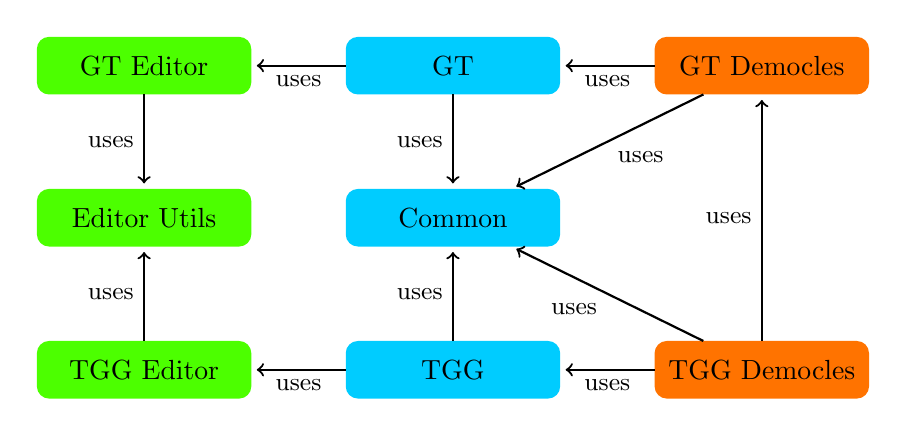
\begin{tikzpicture} [
		auto,
		node/.style = {
			rectangle,
			rounded corners,
			thick,
			text width = 7em,
			text centered,
			minimum height = 2em,
		},
		line/.style = {
			draw,
			thick,
			->,
			shorten >=2pt,
		},
		line-caption/.style = {
			font = \small,
		},
		ibex-ui/.style = {
			draw = green!60!lime,
			fill = green!60!lime,
		},
		ibex/.style = {
			draw = blue!20!cyan,
			fill = blue!20!cyan,
		},
		ibex-democles/.style = {
			draw = red!10!orange,
			fill = red!10!orange
		}
	]

	\matrix[
		column sep = 12mm,
		row sep = 12mm
	] {
		\node[node, ibex-ui] (uiGT) {
			GT Editor
		};
		& \node[node, ibex](GT) {
			GT
		};
		& \node[node, ibex-democles](democlesGT) {
			GT Democles
		};
		\\
		\node[node, ibex-ui] (uiCommon) {
			Editor Utils
		};
		& \node[node, ibex](common) {
			Common
		};
		\\
		\node[node, ibex-ui] (uiTGG) {
			TGG Editor
		};
		& \node[node, ibex](TGG) {
			TGG
		};
		& \node[node, ibex-democles](democlesTGG) {
			TGG Democles
		};
		\\
	};

	\begin{scope} [
		every path/.style = line,
		every node/.style = line-caption
		]
		\path (uiGT) -- node[left] {uses} (uiCommon);
		\path (uiTGG) -- node[left] {uses} (uiCommon);

		\path (GT) -- node {uses} (uiGT);
		\path (TGG) -- node {uses} (uiTGG);

		\path (GT) -- node[left] {uses} (common);
		\path (TGG) -- node[left] {uses} (common);

		\path (democlesGT) -- node {uses} (GT);
		\path (democlesGT) -- node {uses} (common);
		\path (democlesTGG) -- node {uses} (common);
		\path (democlesTGG) -- node {uses} (TGG);
		\path (democlesTGG) -- node {uses} (democlesGT);
	\end{scope}
\end{tikzpicture}

	\caption[Component Diagram for eMoflon::IBeX]{Component Diagram for eMoflon::IBeX (see Appendix~\ref{appendix-list-of-projects} for details)}
	\label{fig:emoflon-ibex-components}
\end{figure}

\noindent
The Common project defines the meta-model for IBeX pattern model, a pattern network which is independent from a concrete pattern matcher.
Currently IBeX patterns are used for GT only, but shall be shared with the TGG part later.
In addition, some utilities for dealing with EMF models are provided.

The GT and TGG projects provide Eclipse integration and runtime code which is independent from a concrete pattern matcher.
To use eMoflon::IBeX, an adapter for a concrete incremental pattern matching engine is necessary.
Currently only Democles \cite{Democles} is fully supported, although prototypes for Viatra and Drools exist.


\section{Transformation of Graph Transformation Rules into IBeX Patterns}
\label{ibex-patterns}
This section explains the transformation from the textual specification in the editor into IBeX patterns which can be understood by a pattern matching engine after another transformation into the pattern format of the engine.
In the following, patterns and rules will be given by their textual syntax and graphical visualization.
The interested reader is referred to the handbook \cite{eMoflonIBeX-GT-Handbook} for more details about the textual syntax.

Figure~\ref{fig:model-transformations} illustrates the use of model transformations in the eMoflon::IBeX implementation.
The user specifies patterns and rules in text files with the file extension \texttt{gt} using an Xtext-based editor.
Xtext automatically parses the file and transforms the textual specification into an editor model when a \texttt{gt} file is loaded.

The visualizations of the editor model, the IBeX patterns, and the Democles patterns are realized via transformations to PlantUML code, which is interpreted and displayed by the PlantUML Eclipse plugin.

\begin{figure}[h!]
	\centering
	% !TeX encoding = UTF-8
% !TeX spellcheck = en_US

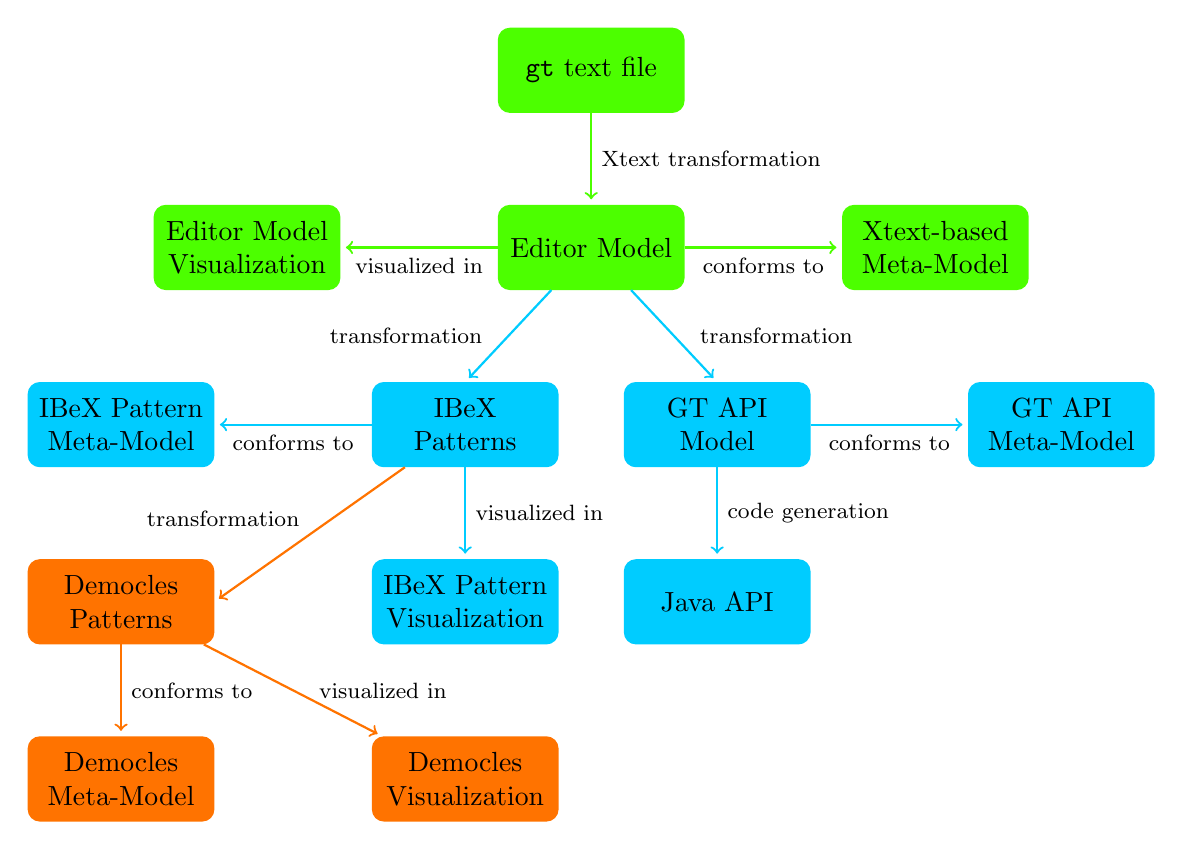
\begin{tikzpicture} [
		auto,
		node distance = 2.25cm,
		node/.style = {
			rectangle,
			rounded corners,
			thick,
			text width = 6em,
			text centered,
			minimum height = 3em,
		},
		line/.style = {
			draw,
			thick,
			->,
			shorten >=2pt,
		},
		line-caption/.style = {
			font = \footnotesize
		},
		ibex-ui/.style = {
			draw = green!60!lime,
			fill = green!60!lime,
		},
		ibex/.style = {
			draw = blue!20!cyan,
			fill = blue!20!cyan,
		},
		ibex-democles/.style = {
			draw = red!10!orange,
			fill = red!10!orange
		}
	]

	\node[node, ibex-ui] (f) {
		\texttt{gt} text file
	};

	\node[node, ibex-ui, below of = f] (e) {
		Editor Model
	};
	\node[node, ibex-ui, left = 2cm of e] (ev) {
		Editor Model Visualization
	};
	\node[node, ibex-ui, right = 2cm of e] (em) {
		Xtext-based Meta-Model
	};

	\node[node, ibex, below of = e, xshift = 1.6cm] (g) {
		GT API Model
	};
	\node[node, ibex, right = 2cm of g] (gm) {
		GT API Meta-Model
	};
	\node[node, ibex, below of = g] (gc) {
		Java API
	};

	\node[node, ibex, below of = e, xshift = -1.6cm] (i) {
		IBeX Patterns
	};
	\node[node, ibex, left = 2cm of i] (im) {
		IBeX Pattern Meta-Model
	};
	\node[node, ibex, below of = i] (iv) {
		IBeX Pattern Visualization
	};

	\node[node, ibex-democles, below of = im] (d) {
		Democles Patterns
	};
	\node[node, ibex-democles, below of = d] (dm) {
		Democles Meta-Model
	};
	\node[node, ibex-democles, below of = iv] (dv) {
		Democles Visualization
	};

	\begin{scope} [
			every path/.style = line, ibex-ui,
			every node/.style = line-caption
		]
		\path (f) -- node[right] {Xtext transformation} (e);
		\path (e) -- node[below] {visualized in} (ev);
		\path (e) -- node[below] {conforms to} (em);
	\end{scope}

	\begin{scope} [
			every path/.style = line, ibex,
			every node/.style = line-caption
		]
		\path (e) -- node[left, xshift = -0.2cm] {transformation} (i.north);
		\path (e) -- node[right, xshift = 0.2cm] {transformation} (g.north);

		\path (i) -- node[below] {conforms to} (im);
		\path (i) -- node[right] {visualized in} (iv);

		\path (g) -- node[below] {conforms to} (gm);
		\path (g) -- node[right] {code generation} (gc);
	\end{scope}

	\begin{scope} [
			every path/.style = line, ibex-democles,
			every node/.style = line-caption
		]
		\path (i) -- node[left, yshift = 0.2cm] {transformation} (d.east);
		\path (d) -- node[right] {conforms to} (dm);
		\path (d) -- node[right, xshift = 0.2cm] {visualized in} (dv);
	\end{scope}
\end{tikzpicture}

	\caption{Model transformations for eMoflon::IBeX-GT}
	\label{fig:model-transformations}
\end{figure}

\noindent
Whenever a project with \texttt{gt} files is built, the editor models of all \texttt{gt} files in a package are transformed into the GT API model and the IBeX pattern model.
In addition, code for a typed Java API is generated as described in Section~\ref{api-code-generation}.

For each pattern and each rule a context pattern containing all context elements, deleted elements, and attribute conditions is generated.
In addition, for each rule a create and a delete pattern is generated to define which elements must be created or deleted when the rule is applied.
The create pattern contains all created nodes and references, together with any attribute assignments, while a delete pattern contains just deleted nodes and references.
Figure~\ref{fig:editor-model-to-IBeXPatterns} summarizes which parts of the editor model are included in which kind of the generated IBeX patterns.

\begin{figure}[h!]
	\centering
	\input{../common/tikz/editor-model-to-IBeXPatterns.tex}
	\caption{Editor model to IBeX patterns}
	\label{fig:editor-model-to-IBeXPatterns}
\end{figure}

\noindent
The transformation from IBeX context patterns to the pattern representation used by a concrete incremental pattern matching engine (\eg Democles) happens at runtime.
If one wants to use eMoflon::IBeX with another pattern matcher, just the orange part in Figure~\ref{fig:model-transformations} (the Democles adapter) needs to be implemented for the other engine, as just this part depends on the meta-model for Democles patterns.

\subsection{Nodes and References}
A pattern/rule consists of nodes and references between them.
Each node and reference must have a type from an Ecore meta-model.
The type of a node can be abstract -- except if the node is created and the rule is not abstract (cp. Section~\ref{pattern-refinement}).
This ensures that all created nodes in applicable rules have a concrete type such that the node can be actually created, which would not be possible for an abstract type.

For each node and reference an operator defines whether it is context (shown with black background in the visualization), created (green) or deleted (red).
Note that some combinations of node and reference operator do not make sense and are forbidden, \eg there must not be a context reference in a created node as there cannot be a reference in a node which does not exist yet.

The pattern \texttt{findCharacterOnExit} (Figure~\ref{fig:pattern-findCharacterOnExit}) will match any characters standing on an exit platform.
The rule \texttt{createCharacter} (Figure~\ref{fig:rule-createCharacter}) which creates a new character and references from the character to an existing game and to an existing platform.
The rule \texttt{moveCharacterToNeighboringPlatform} (Figure~\ref{fig:rule-moveCharacterToNeighboringPlatform}) deletes the \texttt{standsOn} reference between a character to its current platform and creates a new \texttt{standsOn} reference to another platform which must be a neighbor of the previous one.

\begin{figure}[h!]
	\centering
	\subfloat[Textual Syntax]{
		\includegraphics{../common/figures/pattern-findCharacterOnExit-textual}
	}
	\quad
	\subfloat[Visualization]{
		\includegraphics[scale=0.7]{../common/figures/pattern-findCharacterOnExit}
	}
	\caption{Pattern \texttt{findCharacterOnExit}}
	\label{fig:pattern-findCharacterOnExit}
\end{figure}

\begin{figure}[h!]
	\centering
	\subfloat[Textual Syntax]{
		\includegraphics{../common/figures/rule-createCharacter-textual}
	}
	\quad
	\subfloat[Visualization]{
		\includegraphics[scale=0.7]{../common/figures/rule-createCharacter}
	}
	\caption{Rule \texttt{createCharacter}}
	\label{fig:rule-createCharacter}
\end{figure}

\begin{figure}[h!]
	\centering
	\subfloat[Textual Syntax]{
		\includegraphics{../common/figures/rule-moveCharacterToNeighboringPlatform-textual}
	} \\
	\subfloat[Visualization]{
		\includegraphics[scale=0.7]{../common/figures/rule-moveCharacterToNeighboringPlatform}
	}
	\caption{Rule \texttt{moveCharacterToNeighboringPlatform}}
	\label{fig:rule-moveCharacterToNeighboringPlatform}
\end{figure}

\noindent
In eMoflon::IBeX matches must be injective, \ie nodes with different names must be matched to different objects in a match. 
For example, the two platforms in the rule \texttt{moveCharacterToNeighboringPlatform} must be different platforms.
So a platform which has a \texttt{neighbors} edge to itself would not be a valid match.
The decision for injectivity per default has been made as this is what the user intuitively expects when looking at the visualization.
If one does not want to have injectivity for a pattern, one has to specify different variants of the pattern.

A match for a pattern contains all nodes of that pattern -- except so-called local nodes.
Per convention in eMoflon::IBeX-GT, a node is local if and only if its name starts with an underscore.
If one was not interested in the platforms of Figure~\ref{fig:rule-moveCharacterToNeighboringPlatform}, one could name them \texttt{\_platform1} and \texttt{\_platform2} to omit them from in the matches for the pattern.
So local nodes can be used to get smaller matches, as less elements are contained in the match.
As the binding of local nodes is not relevant for the match, specifying nodes as local can reduce the number of matches because different bindings for the local nodes do not result in different matches.

\subsection{Attribute Assignments and Conditions}
Attribute assignments define new attribute values to be set when the rule is applied, 
while attribute conditions are a match filter based on a comparison of attribute values according to the defined relation (\texttt{==}, \texttt{!=}, \texttt{<=}, \texttt{<}, \texttt{>}, or \texttt{>=}).
eMoflon::IBeX-GT supports constants, the attributes of other nodes, and parameters as attribute values as long as the type of the value fits to the one of the attribute.
For example, a String attribute can only have a String value.

\begin{figure}[h!]
	\centering
	\subfloat[Textual Syntax]{
		\includegraphics{../common/figures/pattern-findCharacterOfColor-textual}
	}
	\quad
	\subfloat[Visualization]{
		\includegraphics[scale=0.7]{../common/figures/pattern-findCharacterOfColor}
	}
	\caption{Pattern \texttt{findCharacterOfColor(color: COLOR)}}
	\label{fig:pattern-findCharacterOfColor}
\end{figure}

\begin{figure}[h!]
	\centering
	\subfloat[Textual Syntax]{
		\includegraphics{../common/figures/rule-createBlueCharacter-textual}
	}
	\quad
	\subfloat[Visualization]{
		\includegraphics[scale=0.7]{../common/figures/rule-createBlueCharacter}
	}
	\caption{Rule \texttt{createBlueCharacter}}
	\label{fig:rule-createBlueCharacter}
\end{figure}

\noindent
The pattern \texttt{findColoredCharacter} (Figure~\ref{fig:pattern-findCharacterOfColor}) searches for a character which stands on a platform and has a certain color.
The attribute condition defines that only characters whose color attribute equals the value of the parameter \texttt{color} of the type \texttt{COLOR} (an enum defined in the meta-model) can be matched.
The rule \texttt{createBlueCharacter} (Figure~\ref{fig:rule-createBlueCharacter}) creates a new character whose color attribute is set to \texttt{BLUE}, given by an enum literal.
Attributes which are not specified for created nodes are set to the default value defined in the Ecore meta-model.

Parameters for primitive data types and enums must be declared in the signature of a pattern or a rule.
At run time they are replaced with a concrete value of the correct type.\footnote{Section~\ref{api-parameters} explains how parameters can be passed via the API.}
As parameter values are only bound at run time, parameterized attribute conditions cannot be transformed to Democles, but are handled by the graph transformation interpreter.

Note that there are some logical restrictions when using attribute assignments and conditions:
Attribute assignments must not be placed in deleted nodes (if the node was deleted, its attributes cannot be changed anymore) and conditions cannot occur within created nodes (the node does not exist yet and does not have any attribute values).

\subsection{Applications Conditions}
\label{application-conditions}
Application conditions are additional constraints on graph structures to check when finding matches for a certain pattern:
The application conditions must be fulfilled for the match according to Definitions~\ref{def:satisfaction-of-graph-conditions} and~\ref{def:satisfaction-of-complex-graph-conditions}, otherwise the match is not valid.
eMoflon::IBeX-GT allows to specify positive and negative application conditions and combine them via logical expressions \texttt{\&\&} (logical conjunction) and \texttt{||} (logical disjunction).

By convention, nodes of the same name in a pattern and the patterns used in its application conditions must be matched to the same node.
The arrows in the visualization illustrate which nodes of the different patterns must be equal.
Only the nodes of the main pattern are included in matches, any bindings of the nodes in the patterns of conditions will not be available in matches.

\subsubsection{Negative Application Conditions}
Via \texttt{forbid} a negative application condition (NAC) can be defined.
A NAC invalidates matches with a certain pattern structure.
For example, the pattern \texttt{findEmptyExit} (Figure~\ref{fig:pattern-findEmptyExit}) contains a NAC to ensure that no character stands on the exit platform of the main pattern.
Otherwise any exit platform could be mapped for the \texttt{exit} node regardless of whether characters stand on it or not.

\begin{figure}[h!]
	\centering
	\subfloat[Textual Syntax]{
		\includegraphics{../common/figures/pattern-findEmptyExit-textual}
	}
	\caption{Pattern \texttt{findEmptyExit}}
	\label{fig:pattern-findEmptyExit}
\end{figure}

\begin{figure}[h!]
	\centering
	\ContinuedFloat
	\subfloat[Visualization]{
		\includegraphics[scale=0.7]{../common/figures/pattern-findEmptyExit}
	}
	\caption[]{Pattern \texttt{findEmptyExit} (cont.)}
\end{figure}

\begin{figure}[h!]
	\centering
	\subfloat[Textual Syntax]{
		\includegraphics{../common/figures/pattern-findStandalonePlatform-textual}
	}
	\caption{Pattern \texttt{findStandalonePlatform}}
	\label{fig:pattern-findStandalonePlatform}
\end{figure}

\begin{figure}[h!]
	\ContinuedFloat
	\centering
	\subfloat[Visualization]{
		\includegraphics[scale=0.7]{../common/figures/pattern-findStandalonePlatform}
	}
	\caption[]{Pattern \texttt{findStandalonePlatform} (cont.)}
\end{figure}

\noindent
Multiple application conditions can be combined via \texttt{\&\&} as illustrated in the pattern \texttt{findStandalonePlatform} (Figure~\ref{fig:pattern-findStandalonePlatform}).
The two NACs restrict the matches for the simple platforms such that all platforms which are connected to another platform via a bridge or a wall are excluded as well as any platforms with a neighboring platform.
Platforms matched by the pattern \texttt{findStandalonePlatform} cannot be left by a character standing on it.
When a She Remembered Caterpillars world is created, such a standalone platform with a character standing on it should be avoided, otherwise the game cannot be finished.

\subsubsection{Positive Application Conditions}
The pattern \texttt{findPlatformWithExactlyOneNeighbor} (Figure~\ref{fig:pattern-findPlatformWithExactlyOneNeighbor}) uses a positive application condition (PAC) via \texttt{enforce} in combination with a NAC.
The PAC ensures that the platform must have at least one neighboring platform and the NAC excludes any platforms which have at least two neighbors.
Finally, only the platforms with exactly one neighbor remain as matches.

In this example, the PAC could be simply integrated into the main pattern without changing its meaning.
However, in general PACs are necessary to express certain constraints:
For example, multiple PACs combined via disjunction cannot be expressed with the integration into the main pattern (cp. example in Section \ref{disjunctions}).
In addition, the nodes used in application conditions are not contained in the matches.

\begin{figure}[h!]
	\centering
	\subfloat[Textual Syntax]{
		\includegraphics{../common/figures/pattern-findPlatformWithExactlyOneNeighbor-textual}
	} \\
	\subfloat[Visualization]{
		\includegraphics[scale=0.7]{../common/figures/pattern-findPlatformWithExactlyOneNeighbor}
	}
	\caption{Pattern \texttt{findPlatformWithExactlyOneNeighbor}}
	\label{fig:pattern-findPlatformWithExactlyOneNeighbor}
\end{figure}

\subsubsection{Disjunctions}
\label{disjunctions}
Application conditions can be used to express alternatives as well:
For example,
the pattern \texttt{findPlatformWithTwoWays} (Figure~\ref{fig:pattern-findPlatformWithTwoWays}) searches for platforms which have at least two ways to enter or leave the platform (either via neighboring platforms or via bridges/walls).
To express this, three application conditions need to be combined via \texttt{||} to deal with the possibilities that the platform 
(1) has two neighboring platforms,
(2) has two connections to bridges or walls,
or (3) one neighboring platform and one connection to a bridge or a wall.

\begin{figure}[h!]
	\centering
	\subfloat[Textual Syntax]{
		\includegraphics{../common/figures/pattern-findPlatformWithTwoWays-textual}
	}
	\caption{Pattern \texttt{findPlatformWithTwoWays}}
	\label{fig:pattern-findPlatformWithTwoWays}
\end{figure}

\begin{figure}
	\ContinuedFloat
	\centering
	\subfloat[Visualization]{
		\includegraphics[width=\linewidth, trim=8mm 0 0 0]{../common/figures/pattern-findPlatformWithTwoWays-ltr}
	}
	\caption[]{Pattern \texttt{findPlatformWithTwoWays} (cont.)}
\end{figure}

\noindent
In the IBeX pattern model, patterns with multiple disjunctions are represented as a set of alternative patterns.
A match for the pattern is defined as a match for any of the alternative patterns.
For each alternative pattern a separate pattern is generated which is given to the pattern matching engine because Democles cannot deal with alternatives directly (although this feature is planned for the future).
As usual, Democles reports the matches for all patterns to the graph transformation interpreter, which has to collect and combine the matches of all alternative patterns, excluding duplicate matches.
The removal of duplicates is necessary as Democles may report the same match for multiple alternative patterns.

The three alternatives for the pattern \texttt{findPlatformWithTwoWays} are disjoint.
So no matches will be removed when combining the matches of the three alternatives because no duplicates can be found.
Without the NACs in the third alternative, a match for a platform with two neighbors and a bridge connection (as the platform \texttt{p1} shown in Figure~\ref{fig:example-model-duplicate-matches}) would be reported by the first and the third alternative.
The duplicate check would remove one of the matches, so the interpreter would still return the same set of matches.
Without the removal of matches, a match reported by two alternatives would be returned twice.

\begin{figure}[h!]
	\centering
	\begin{tikzpicture}
		\node[tnode] (p1) {p1: SimplePlatform};
		\node[tnode, below = of p1] (p2) {p2: SimplePlatform};
		\node[tnode, left = of p2] (b) {b: Bridge};
		\node[tnode, right = of p2] (p3) {p3: SimplePlatform};
		
		\draw[tedge] (p1.west) -- (b);
		\draw[tedge] (p2) -- (b);
		\draw[tedge] (p1) -- (p2);
		\draw[tedge] (p1) -- (p3);
	\end{tikzpicture}
	\caption{Example Model with Matches Reported for Two Alternatives}
	\label{fig:example-model-duplicate-matches}
\end{figure}

\noindent
Note that logical expressions combining application conditions must be given in disjunctive normal form (DNF), \ie the clauses combined via \texttt{||} must only contain PACs and NACs combined via \texttt{\&\&}.
This is necessary to easily create the alternative patterns which can be given to the pattern matcher, as for each clause an alternative pattern is generated, containing the main pattern with the PACs and NACs from the clause.

\subsection{Pattern Refinement}
\label{pattern-refinement}
Pattern refinement is a modularity concept on the level of patterns which allows to share common subparts of the pattern with one or multiple super patterns.
Similar to inheritance in object-oriented programming, this avoids declaring the same graph structures in multiple patterns.
So pattern refinement helps to reduce copy and paste and leads to a specification which can be maintained more easily.

Patterns with super patterns are flattened, \ie transformed into an equivalent version without pattern refinement.
After that the flattened pattern is transformed into IBeX patterns as shown in Figure~\ref{fig:editor-model-to-IBeXPatterns}.
The semantics of pattern refinement (how a pattern with super patterns can be flattened) is given by Definition~\ref{def:refined-pattern}.\footnote{The definition of rule refinement for Triple Graph Grammars by Stolte \cite{ExploitingTheModularityOfTGGs} is generalized for graph transformations.}
Note that application conditions are not inherited to avoid additional complexity in situations in which the application conditions of super patterns come into conflict with each other.
Due to this decision the user cannot lose track of the application conditions of a concrete pattern.

Patterns can be abstract: Abstract means that the pattern cannot be applied directly, but only exists to be used as a super pattern.

\newpage % Without this line LaTeX puts a pagebreak after the first line of the definition.
\begin{definition}[Refined Pattern]
	\label{def:refined-pattern}%
	A pattern with one or more super patterns is called a \textit{refined pattern}.
	The semantics of such a pattern is defined by the following constraints:
	\begin{enumerate}
		\item A pattern contains all nodes from its super patterns.
		\item Equivalent nodes (identified by their name) are merged into one node.
		\item Equivalent references (identified by their type, source and target node) are merged into one edge.
		\item Equivalent attribute assignments (identified by their node, attribute type and value) are merged into one attribute assignment.
			There must not be different attribute assignments for the same attribute inherited from different patterns.
		\item Equivalent attribute conditions (identified by their node, attribute type, relation and value) are merged into one attribute condition.
		\item Equivalent parameters (identified by their name) are merged into one parameter.
			There must not be different type definitions for parameters of the same name.
		\item When overriding a node/reference, created/deleted elements can be overwritten by context elements.
			Context elements must not be overwritten by created or deleted elements.
			Created elements must not be overwritten by deleted elements, deleted elements must not be overwritten by created elements.
		\item The type of a node is the lowest of the types of all declarations of a node within a pattern and its super patterns.
			The type of a node can only be the same type or a lower type as declared for a node of the same name in a super pattern.
	\end{enumerate}
\end{definition}

\noindent
Table~\ref{table:node-type-changes} shows some combinations of allowed and forbidden node type declarations in refined patterns and their super patterns according to the last constraint.
Specifications without a lowest type and type not conforming to the type in the super pattern lead to an error message in the editor.

\begin{longtable}[h!]{lll}
	\toprule
	Node types in super patterns
		& Node type in pattern
		& Final type \\
	\midrule
	Platform
		& \text{(none)}
		& Platform \\
	Platform, SimplePlatform
		& (none)
		& SimplePlatform \\
	ExitPlatform, SimplePlatform
		& (none)
		& ERROR (no lowest type) \\
	ExitPlatform
		& Platform
		& ERROR (no subtype) \\
	Platform
		& SimplePlatform
		& SimplePlatform \\
	ExitPlatform
		& SimplePlatform
		& ERROR (no subtype) \\
	\bottomrule
	\caption{Allowed and Forbidden Node Type Changes in Refined Patterns}
	\label{table:node-type-changes}
\end{longtable}

\begin{figure}[h!]
	\centering
	\subfloat[Textual Syntax]{
		\includegraphics{../common/figures/rules-moveCharacter-textual}
		\label{fig:rules-moveCharacter-textual}
	}
	\caption{Rules with Refinements}
	\label{fig:examples-with-refinement}
\end{figure}

\begin{figure}[h!]
	\ContinuedFloat
	\centering
	\subfloat[Refinement Hierarchy]{
		\includegraphics{../common/figures/pattern-refinement-hierarchy-moveCharacter}
		\label{fig:pattern-refinement-hierarchy-moveCharacter}
	} \\
	\subfloat[Abstract Rule \texttt{moveCharacter}]{
		\includegraphics[scale=0.7]{../common/figures/rule-moveCharacter}
		\label{fig:rule-moveCharacter}
	}
	\subfloat[Rule \texttt{moveCharacterToNeighboringPlatform}]{
		\includegraphics[scale=0.7]{../common/figures/rule-moveCharacterToNeighboringPlatform}
		\label{fig:rule-moveCharacterToNeighboringPlatform2}
	}
	\caption[]{Rules with Refinements (cont.)}
\end{figure}

\noindent
Figure~\ref{fig:examples-with-refinement} shows some rules having a lot of elements in common.
Using the pattern refinement hierarchy shown in Figure~\ref{fig:pattern-refinement-hierarchy-moveCharacter}, duplications in the textual specification can be avoided or at least significantly reduced as only nodes with additional references or another type need to be redeclared in the refined pattern.
Nodes which are already defined in a super pattern are highlighted in bold.
The visualization shows the refined rules after the flattening according to Definition~\ref{def:refined-pattern}.

The rule \texttt{moveCharacterToNeighboringPlatform} just specifies the \texttt{neighbors} edge between the two platforms, all objects and the other edges are inherited from the super rule \texttt{moveCharacter}.
The abstract rule \texttt{moveCharacterAcrossPlatformConnector} overrides the type of the platform nodes to a subtype, \texttt{SimplePlatform}.
The rules \texttt{moveCharacterAcrossBridge} and \texttt{moveCharacterOverWall} define that the two platforms must be connected via a bridge or a wall, respectively.

\begin{figure}[h!]
	\ContinuedFloat
	\centering
	\subfloat[Abstract Rule \texttt{moveCharacterAcrossPlatformConnector}]{
		\includegraphics[scale=0.7]{../common/figures/rule-moveCharacterAcrossPlatformConnector}
		\label{fig:rule-moveCharacterAcrossPlatformConnector}
	} \\
	\subfloat[Rule \texttt{moveCharacterAcrossBridge}]{
		\includegraphics[scale=0.7]{../common/figures/rule-moveCharacterAcrossBridge}
		\label{fig:rule-moveCharacterAcrossBridge}
	} \\
	\subfloat[Rule \texttt{moveCharacterOverWall}]{
		\includegraphics[scale=0.7]{../common/figures/rule-moveCharacterOverWall}
		\label{fig:rule-moveCharacterOverWall}
	}
	\caption[]{Rules with Refinements (cont.)}
\end{figure}

The algorithm for the flattening of an editor pattern collects all nodes of the pattern and its super patterns and combines them into one large pattern (so-called co-product).
After that parts which are equivalent according to Definition~\ref{def:refined-pattern} are merged as described in the following:

\begin{enumerate}
	\item When merging two nodes, the operator is given by Table~\ref{table:merging-operators} (see constraint 7 in the definition) and the type of the node is the lower type of the two merged nodes.
		In the case that two nodes of the same name have different types and none of the types is a subtype of the other, the specification is invalid.
	\item When merging two equivalent references, attribute assignments, or attribute conditions only one of them remains and the other one is removed.
		\begin{enumerate}
			\item The operator of merged references is given by Table~\ref{table:merging-operators}.
			\item If there are multiple attribute assignments for the same attribute within a node, their values must be equal.
				Otherwise the specification is invalid, as one cannot decide which attribute value shall be assigned.
		\end{enumerate}
	\item When merging parameters, the parameters of the super patterns are appended to the parameter list of the refined pattern.
		If parameters of the same name have different types, the specification is invalid.
\end{enumerate}

\begin{longtable}[h!]{c|ccc}
	\toprule
				& \create	& \delete 	& context \\
	\midrule
	\create		& \create	& ERROR		& context \\
	\delete		& ERROR		& \delete	& context \\
	context		& context	& context	& context \\
	\bottomrule
	\caption{Operators of Merged Nodes and References in Refined Patterns}
	\label{table:merging-operators}
\end{longtable}

\noindent
For the flattening algorithm it is irrelevant whether a node is specified in the refined pattern or one of its super patterns.
Only for parameters the order is relevant (because the parameters of the pattern specification become parameters for the constructor of the pattern).
By repeating all parameters in the refined pattern, the user can influence the order of all parameters.

The user gets feedback on invalid specifications by error markers shown in the editor.
When a project with invalid specifications is built, the problems are written on the console.


\section{Pattern Networks}
\label{pattern-networks}
The previous sections introduced the features of the pattern language in the textual editor: nodes and references, attributes, application conditions, and pattern refinement.
This section gives a summary how they are represented in the editor model, the IBeX pattern model, and in Democles.
In addition, details on the transformations are provided.

The parser of the Xtext framework parses \texttt{gt} files into an editor model file containing \texttt{EditorPattern}s and \texttt{EditorCondition}s.
Figure~\ref{fig:editor-patterns-meta-model} shows a simplified class diagram of the editor model.
\texttt{EditorPattern}s have a type, either \texttt{PATTERN} or \texttt{RULE}.
By using the same object for patterns and rules, both can easily be used together in a refinement hierarchy.
They consist of a set of \texttt{EditorNode}s, which can have \texttt{EditorAttribute}s and \texttt{EditorReference}s.
An \texttt{EditorAttribute} has a relation (assignment or a comparison such as equals) and an attribute value.
An \texttt{EditorReference} has a target node.

Both \texttt{EditorNode}s and \texttt{EditorReference}s have an operator, either \texttt{CONTEXT} (default value), \texttt{CREATE} (keyword \create~in the editor), or \texttt{DELETE} (\delete).

\texttt{EditorPattern}s have a set of \texttt{EditorCondition}s (disjunction).
\texttt{EditorCondition}s represent a conjunction of conditions (a clause in the DNF), which can be a reference to another \texttt{EditorCondition} or a positive or negative \texttt{EditorApplicationCondition} (\texttt{enforce} or \texttt{forbid}).
\texttt{EditorConditionReference} reference another condition.

\begin{figure}[H]
	\centering
	% !TeX encoding = UTF-8
% !TeX spellcheck = en_US

\begin{tikzpicture}
	\umlsimpleclass[class]
		{EditorPattern}

	% classes for conditions
	\umlsimpleclass[class,
		below = 1.5cm of EditorPattern,
		xshift = -2cm]
		{EditorCondition}
	\umlsimpleclass[class,
		below = 1.5cm of EditorCondition]
		{EditorSimpleCondition}
	\umlsimpleclass[class,
		below = 2.25cm of EditorSimpleCondition,
		xshift = 2cm]
		{EditorConditionReference}
	\umlsimpleclass[class,
		below = 1cm of EditorSimpleCondition,
		xshift = -2cm]
		{EditorApplicationCondition}

	% classes node, attribute and reference
	\umlsimpleclass[class,
		below = 1.5cm of EditorPattern,
		xshift = 4.25cm]
		{EditorNode}
	\umlsimpleclass[class,
		below = 1.5cm of EditorNode,
		xshift = -1.8cm]
		{EditorAttribute}
	\umlsimpleclass[class,
		below = 1.5cm of EditorNode,
		xshift = 1.8cm]
		{EditorReference}

	% EditorPattern
	\umluniassoc[arg2 = {superPatterns},
		mult2 = 0..*,
		pos = 0.5,
		angle1 = 90,
		angle2 = 0,
		loopsize = 2cm]
		{EditorPattern}
		{EditorPattern}
	\umluniassoc[geometry=|-|,
		arg2 = {conditions (OR)},
		mult2 = 0..*,
		pos2 = 2.5,
		anchor1 = -130,
		anchor2 = 90]
		{EditorPattern}
		{EditorCondition}
	\umlunicompo[geometry = |-|,
		arg2 = {nodes},
		mult2 = 0..*,
		pos = 2.5,
		anchor1 = -50,
		anchor2 = 90]
		{EditorPattern}
		{EditorNode}

	% EditorNode
	\umlunicompo[geometry = |-|,
		arg2 = {attributes},
		mult2 = 0..*,
		pos = 2.5,
		anchor1 = -130]
		{EditorNode}
		{EditorAttribute}
	\umlunicompo[geometry = |-|,
		arg2 = {references},
		mult2 = 0..*,
		pos = 2.5,
		anchor1 = -50,
		anchor2 = 90]
		{EditorNode}
		{EditorReference}

	% EditorReference
	\umluniassoc[geometry = -|-,
		arg2 = {target},
		mult2 = 1,
		pos = 2.5,
		anchor1 = 0,
		anchor2 = 0,
		arm1 = 0.5cm]
		{EditorReference}
		{EditorNode}

	% EditorCondition
	\umlunicompo[arg2 = {conditions (AND)},
		mult2 = 1..*,
		pos2 = 0.75]
		{EditorCondition}
		{EditorSimpleCondition}

	% EditorConditionReference
	\umlinherit[geometry = |-|,
		anchor1 = 125,
		anchor2 = -20]
		{EditorConditionReference}
		{EditorSimpleCondition}
	\umluniassoc[geometry = |-|,
		arm1 = 1.5cm,
		arg2 = {condition},
		mult2 = 1,
		pos2 = 1.45,
		anchor1 = 12,
		anchor2 = -12]
		{EditorConditionReference}
		{EditorSimpleCondition}

	% EditorApplicationCondition
	\umlinherit[geometry = |-|,
		anchor2 = -135]
		{EditorApplicationCondition}
		{EditorSimpleCondition}
	\umluniassoc[geometry = |-,
		arg2 = {pattern},
		mult2 = 1,
		pos = 1.5,
		anchor1 = 170,
		anchor2 = 180]
		{EditorApplicationCondition}
		{EditorPattern}
\end{tikzpicture}

	\caption{Simplified Meta-Model of the Editor Model}
	\label{fig:editor-patterns-meta-model}
\end{figure}

\subsection{IBeX Pattern Networks}
\label{ibex-pattern-networks}
During the build of a graph transformation project in Eclipse with eMoflon::IBeX, the editor specification is transformed into the IBeX pattern model, which is saved in an \texttt{ibex-patterns.xmi}.
Just this file is used by the graph transformation interpreter and must be read at runtime.

A simplified class diagram for the IBeX pattern model (just context patterns) is shown in Figure~\ref{fig:ibex-patterns-meta-model}.
An \texttt{IBeXContextPattern} consists of signature nodes, local nodes and edges, injectivity constraints, attribute constraints, and pattern invocations.

Table~\ref{table:ibex-pattern-networks} summarizes how patterns and rules of the editor model are transformed into the IBeX pattern model.
\texttt{EditorPattern}s with no or just one clause in the DNF are transformed into an \texttt{IBeXContextPattern}.
If there are more than two disjunctions, the \texttt{EditorPattern} is transformed into an \texttt{IBeXContextAlternative}s, containing one \texttt{IBeXContextPattern} per clause in the DNF.

Each \texttt{EditorNode} is transformed to an \texttt{IBeXNode}.
If the name of the name starts with an underscore, the node is local (\ie not part of a match), otherwise the node is a signature node.
For each pair of two nodes for which the type declaration does not ensure that the nodes are mapped to different objects, an injectivity constraint is added.
Such a constraint defines a pair of nodes, which must not be equal.

Pattern refinement is not included in the table as the refinement is ``flattened'' and the flattened pattern is transformed afterwards.

\begin{figure}[H]
	\centering
	% !TeX encoding = UTF-8
% !TeX spellcheck = en_US

\begin{tikzpicture}
	\umlsimpleclass[class]
		{IBeXContext}
	\umlsimpleclass[class,
		right = 1.5cm of IBeXContext]
		{IBeXContextAlternatives}
	\umlsimpleclass[class,
		below = 1cm of IBeXContext]
		{IBeXContextPattern}
	\umlsimpleclass[class,
		below = 1.5cm of IBeXContextPattern,
		xshift = -4cm]
		{IBeXPatternInvocation}
	\umlsimpleclass[class,
		below = 1.5cm of IBeXContextPattern,
		xshift = 5cm]
		{IBeXAttributeConstraint}
	\umlsimpleclass[class,
		below = 0.75cm of IBeXAttributeConstraint,
		xshift = 1cm]
		{IBeXNodePair}
	\umlsimpleclass[class,
		below = 1cm of IBeXNodePair]
		{IBeXNode}
	\umlsimpleclass[class,
		below = 2.5cm of IBeXNode]
		{IBeXEdge}

	% IBeXContextAlternatives
	\umlinherit[]
		{IBeXContextAlternatives}
		{IBeXContext}
	\umlunicompo[geometry = |-,
		arg2 = {alternatives},
		mult2 = 2..*,
		pos = 1.5,
		anchor2 = 0]
		{IBeXContextAlternatives}
		{IBeXContextPattern}

	% IBeXContextPattern
	\umlinherit[]
		{IBeXContextPattern}
		{IBeXContext}
	\umlunicompo[geometry = |-|,
		arg2 = {attributeConstraints},
		mult2 = 0..*,
		pos = 2.5,
		anchor1 = -15.2]
		{IBeXContextPattern}
		{IBeXAttributeConstraint}
	\umlunicompo[geometry = |-,
		arg2 = {injectivityConstraints},
		mult2 = 0..*,
		pos = 1.5,
		anchor1 = -25]
		{IBeXContextPattern}
		{IBeXNodePair}
	\umlunicompo[geometry = |-,
		arg2 = {signatureNodes},
		mult2 = 1..*,
		pos = 1.6,
		anchor1 = -55,
		anchor2 = 165]
		{IBeXContextPattern}
		{IBeXNode}
	\umlunicompo[geometry = |-,
		arg2 = {localNodes},
		mult2 = 0..*,
		pos = 1.4,
		anchor1 = -125,
		anchor2 = 195]
		{IBeXContextPattern}
		{IBeXNode}
	\umlunicompo[geometry = |-,
		arg2 = {localEdges},
		mult2 = 0..*,
		pos = 1.4,
		anchor1 = -155]
		{IBeXContextPattern}
		{IBeXEdge}
	\umlunicompo[geometry = |-|,
		arg2 = {invocations},
		mult2 = 0..*,
		pos = 2.5,
		anchor1 = -164.8]
		{IBeXContextPattern}
		{IBeXPatternInvocation}

	% IBeXNodePair
	\umluniassoc[arg2 = {values},
		mult2 = 2,
		pos2 = 0.5]
		{IBeXNodePair}
		{IBeXNode}

	% IBeXEdge -- IBeXNode
	\umlassoc[arg1 = {outgoingEdges},
		mult1 = 0..*,
		pos1 = 0.25,
		align1 = right,
		arg2 = {sourceNode},
		mult2 = 1,
		pos2 = 0.75,
		align2 = right,
		anchor1 = 120,
		anchor2 = -120]
		{IBeXEdge}
		{IBeXNode}
	\umlassoc[arg1 = {incomingEdges},
		mult1 = 0..*,
		pos1 = 0.25,
		align1 = left,
		arg2 = {targetNode},
		mult2 = 1,
		pos2 = 0.75,
		align2 = left,
		anchor1 = 60,
		anchor2 = -60]
		{IBeXEdge}
		{IBeXNode}

	% IBeXPatternInvocation
		\umluniassoc[geometry = -|-,
			arg2 = {invokedPattern},
			mult2 = 1,
			pos = 2.5,
			anchor1 = 180,
			arm1 = 0.5cm]
		{IBeXPatternInvocation}
		{IBeXContextPattern}
\end{tikzpicture}

	\caption{Simplified Meta-Model of the IBeX Pattern Model}
	\label{fig:ibex-patterns-meta-model}
\end{figure}

\begin{longtable}[h!]{p{55mm}p{85mm}}
	\toprule
	Editor model
		& IBeX model \\
	\midrule
	\texttt{EditorNode} (if the operator is \texttt{CONTEXT} or \texttt{DELETE})
		& \texttt{IBeXNode} (as local node if the name starts with \texttt{\_}, otherwise as a signature node)
			and injectivity constraints \\
	\midrule
	\texttt{EditorReference} (if the operator is \texttt{CONTEXT} or \texttt{DELETE})
		& Positive \texttt{IBeXPatternInvocation} of an edge pattern with two signature nodes and one \texttt{IBeXEdge} \\
	\midrule
	\texttt{EditorAttribute} (if the relation is not an assignment)
		& \texttt{IBeXAttributeConstraint} (value given by a constant, a node and an attribute type or a parameter name) \\
	\midrule
	\texttt{EditorApplicationCondition}
		& \texttt{IBeXPatternInvocation} (positive invocation for PACs, negative invocation for NACs) \\
	\bottomrule
	\caption{Transformation from the Editor Model into IBeX Patterns}
	\label{table:ibex-pattern-networks}
\end{longtable}

\noindent
References and application conditions are transformed into so-called pattern invocations.
A pattern invocation is the equivalent to a method call in general programming languages.
It defines that the graph structure of invoked pattern must be matched with the mapping of nodes from the original pattern to the signature nodes of the invoked pattern.
The patterns connected via pattern invocations form a pattern network.

The context pattern generated for the rule \texttt{moveCharacterToNeighboringPlatform} (introduced in the previous section, Figure~\ref{fig:rule-moveCharacter}) is shown Figure~\ref{fig:ibex-pattern-moveCharacterToNeighboringPlatform}.
The main pattern contains only the three nodes.
The left pattern invocation ensures that there must be a \texttt{standsOn} edge between the objects mapped to the signature nodes \texttt{character} and \texttt{platform1} in the main pattern.
\texttt{platform1} and \texttt{platform2} must be connected via a \texttt{neighbors} edge to fulfill the right pattern invocation.

Extracting the edges into edge patterns invoked by the main patterns leads to smaller patterns.
Of course, edge patterns can be invoked by multiple patterns (or even multiple times by the same pattern, using different node mappings).
For example, the edge pattern \texttt{edge-Character-standsOn-Platform} is invoked by all patterns which require a \texttt{standsOn} edge between a character and a platform.

\begin{figure}[h!]
	\centering
	\includegraphics[scale=0.7]{../common/figures/ibex-pattern-moveCharacterToNeighboringPlatform}
	\caption{IBeX Context Pattern \texttt{moveCharacterToNeighboringPlatform}}
	\label{fig:ibex-pattern-moveCharacterToNeighboringPlatform}
\end{figure}

\subsection{Democles Pattern Networks}
\label{democles-pattern-networks}
The meta-model of the pattern network used by Democles is shown in Figure~\ref{fig:democles-patterns-meta-model} (simplified).
A Democles \texttt{Pattern} consists of symbolic parameters and a \texttt{PatternBody}, which contains local variables and constraints.

All elements from the IBeX representation to their equivalent in the Democles model, as shown in Table~\ref{table:pattern-networks}.
As Democles cannot handle parameterized attribute conditions and alternatives of multiple patterns, these two scenarios are handled by the interpreter via filtering and combining (see Section~\ref{api-usage} for detailed information).

\begin{figure}[H]
	\centering
	% !TeX encoding = UTF-8
% !TeX spellcheck = en_US

\begin{tikzpicture}
	\umlsimpleclass[class]
		{Pattern}
	\umlsimpleclass[class,
		below = 1.5cm of Pattern]
		{PatternBody}
	\umlsimpleclass[class,
		below = 1.5cm of PatternBody]
		{Constraint}

	\umlsimpleclass[class,
		below = 1cm of Constraint,
		xshift = -1.5cm]
		{PatternInvocationConstraint}
	\umlsimpleclass[class,
		right = 0.5cm of PatternInvocationConstraint]
		{Reference}
	\umlsimpleclass[class,
		right = 0.5cm of Reference]
		{RelationalConstraint}
	\umlsimpleclass[class,
		below = 1cm of RelationalConstraint]
		{Unequal}
	\umlsimpleclass[class,
		left = 0.5cm of Unequal]
		{Equal}
	\umlsimpleclass[class,
		right = 0.5cm of Unequal,
		alias=x]
		{...}

	\umlsimpleclass[class,
		right = 4cm of Pattern]
		{EMFVariable}
	\umlsimpleclass[class,
		right = 4cm of Constraint]
		{ConstraintParameter}

	\umlunicompo[arg2 = {bodies},
		mult2 = 1..*,
		pos = 0.75]
		{Pattern}
		{PatternBody}
	\umlunicompo[arg2 = {symbolicParameters},
		mult2 = 1..*,
		pos = 0.5]
		{Pattern}
		{EMFVariable}
	\umlunicompo[geometry = -|,
		arg2 = {localVariables},
		mult2 = 0..*,
		pos = 0.5,
		anchor2 = -140]
		{PatternBody}
		{EMFVariable}
	\umlunicompo[arg2 = {constraints},
		mult2 = 0..*,
		pos = 0.75]
		{PatternBody}
		{Constraint}
	\umlunicompo[arg2 = {parameters},
		mult2 = 0..*,
		pos = 0.5]
		{Constraint}
		{ConstraintParameter}
	\umluniassoc[geometry = |-|,
		arg2 = {reference},
		mult2 = 0..*,
		pos = 0.75,
		anchor2 = -40]
		{ConstraintParameter}
		{EMFVariable}

	\umluniassoc[geometry = |-,
		arg2 = {invokedPattern},
		mult2 = 0..*,
		pos = 1.5,
		anchor1 = 170,
		anchor2 = 180]
		{PatternInvocationConstraint}
		{Pattern}

	\umlinherit[geometry=|-|]
		{PatternInvocationConstraint}
		{Constraint}
	\umlinherit[geometry=|-|]
		{RelationalConstraint}
		{Constraint}
	\umlinherit[geometry=|-|]
		{Reference}
		{Constraint}
	\umlinherit[geometry=|-|]
		{Equal}
		{RelationalConstraint}
	\umlinherit[geometry=|-|]
		{Unequal}
		{RelationalConstraint}
	\umlinherit[geometry=|-|]
		{x}
		{RelationalConstraint}
\end{tikzpicture}

	\caption{Simplified Meta-Model for Democles Patterns}
	\label{fig:democles-patterns-meta-model}
\end{figure}

\begin{longtable}[h!]{p{75mm}p{65mm}}
	\toprule
	IBeX model
		& Democles model \\
	\midrule
	\texttt{IBeXNode} as local node
		& \texttt{EMFVariable} as local node \\
	\texttt{IBeXNode} as a signature node
		& \texttt{EMFVariable} as symbolic parameter \\
	\texttt{IBeXAttributeConstraint} (if the value is a constant or an attribute of another node)
		& Subtype of \texttt{RelationalConstraint} (for the correct relation) based on \texttt{EMFVariable}s and constants \\
	Injectivity constraint (\texttt{IBeXNodePair})
		& \texttt{Unequal} constraint \\
	\texttt{IBeXEdge}
		& \texttt{Reference} constraint \\
	\texttt{IBeXPatternInvocation}
		& \texttt{PatternInvocationConstraint} \\
	\bottomrule
	\caption{Transformation from IBeX Patterns into Democles Patterns}
	\label{table:pattern-networks}
\end{longtable}

	% !TeX encoding = UTF-8
% !TeX spellcheck = en_US

\chapter{Graph Transformation Java API}
\label{api}
This chapter describes how a typed Java API can be extracted from the textual specification such that the specified patterns and rules can be invoked from Java code without casting all results and losing type safety (Section~\ref{api-code-generation}).
Section~\ref{gt-interpreter} describes how the API delegates method calls to the graph transformation interpreter, while Section~\ref{api-usage} deals with the usage of the API.
Finally, Section~\ref{incrementality} presents the realization of features which exploit the incrementality of the underlying pattern matcher.

\section{Code Generation for a Typed Java API}
\label{api-code-generation}
The graph transformation specification is placed in a graph transformation project in the Eclipse IDE.\footnote{Any Java and plugin project will be automatically converted to a graph transformation project when adding at least one \texttt{gt} file via the wizard.
	Note that Eclipse projects can have multiple natures: A graph transformation project must have at least the GT, Java and plugin nature.}
All \texttt{gt} files must be placed in the \texttt{src} folder of the project.
For each package containing at least one \texttt{gt} file an API will be generated.
The generated code and models will be placed in corresponding packages in the \texttt{src-gen} folder.

Figure~\ref{fig:api-classes} gives an overview of the API classes assuming there is a package \texttt{example} containing a \texttt{gt} file with a pattern \texttt{ex1()} and a rule \texttt{ex2()}.
For clarity, the class diagram shows only a small subset of the methods implemented by the abstract super classes.
The API serves as a factory for patterns and rules as it provides methods for all non-abstract patterns and rules defined in the package.
The app provides utility methods to create or load EMF resources and add them to the model and initialize the API for a concrete pattern matching engine.
Within the packages \texttt{example.api.rules} and \texttt{example.api.matches} subclasses for the concrete patterns and rules are generated:
\begin{itemize}
	\item The pattern/rule class contains methods for binding context and deleted nodes (except local ones) to a specific object (cp. Section~\ref{api-node-bindings} for more information on node binding).
	If a pattern/rule has parameters (cp. Section~\ref{api-parameters}), they must be initialized in the constructor.
	In addition, setters for all parameters are generated.
	\item The match class contains getters for all nodes in the pattern/rule except the ones marked as local.
\end{itemize}

\noindent
Pattern and rule classes inherit from a super class, \texttt{GraphTransformationPattern} or \texttt{GraphTransformationRule}.
Match classes inherit from \texttt{GraphTransformationMatch}.
These super classes are abstract and implement all methods which are independent from a concrete specification such that only a minimal subset of method implementation needs to be generated.

\begin{figure}[H]
	\centering
	\begin{adjustwidth}{-15mm}{}
		% !TeX encoding = UTF-8
% !TeX spellcheck = en_US

\begin{tikzpicture}
	\begin{umlpackage}[x = 0, y = 0, name=api]{org.emoflon.ibex.gt.api}
		\umlabstract[class, x = 0.8, y = 0]
			{GraphTransformationApp}{
				\# resourceSet: ResourceSet
			}{
				\umlvirt{\# registerMetaModels()} \methodSep
				\umlvirt{\# initAPI(): API}
			}

		\umlabstract[class, x = 0.8, y = -3]
			{GraphTransformationAPI}{}{
				+ getModel(): ResourceSet \methodSep
				+ setDPO() \methodSep
				+ setSPO() \methodSep
				+ updateMatches()
			}

		\umlabstract[class, x = 0.8, y = -7.7]
			{GraphTransformationPattern}{
				\# parameters: Map$<$String, Object$>$
			}{
				\umlvirt{\# convertMatch(IMatch): M} \methodSep
				+ findAnyMatch(): Optional$<$M$>$ \methodSep
				+ findMatches(): Collection$<$M$>$ \methodSep
				+ getParameters(): Map$<$String, Object$>$ \methodSep
				\umlvirt{\# getParameterNames(): List$<$String$>$} \methodSep
				+ subscribeAppearing(Consumer$<$M$>$) \methodSep
				+ subscribeDisappearing(Consumer$<$M$>$) \methodSep
				+ subscribeMatchDisappears(M, Consumer$<$M$>$)
			}

		\umlabstract[class, x = 1.2, y = -12.2]
			{GraphTransformationRule}{}{
				+ apply(): Optional$<$M$>$ \methodSep
				+ setDPO() \methodSep
				+ setSPO()
			}

		\umlabstract[class, x = 1.2, y = -14]
			{GraphTransformationMatch}{}{}
	\end{umlpackage}
	
	\umlinherit
		{GraphTransformationRule}
		{GraphTransformationPattern}
	\umluniassoc[arg2=api, pos2= 0.5]
		{GraphTransformationPattern}
		{GraphTransformationAPI}
	\umluniassoc[arg2=pattern, pos2 = 1.6, align2=right, anchor2 = -132, geometry=-|]
		{GraphTransformationMatch}
		{GraphTransformationPattern}

	\begin{umlpackage}[x = 3.5, y = -17.3, name=engine]{org.emoflon.ibex.gt.engine}
		\umlclass[class, x = 0, y = 0]
			{GraphTransformationInterpreter}{}{
				+ apply(IMatch, PushoutApproach, Map$<$String, Object$>$): Optional$<$IMatch$>$ \methodSep
				+ matchStream(String, Map$<$String, Object$>$): Stream$<$IMatch$>$
			}
	\end{umlpackage}

	\umluniassoc[arg2=interpreter, pos2 = 2, geometry=-|-, arm1=-4.5cm]
		{GraphTransformationAPI}
		{GraphTransformationInterpreter}
	\umluniassoc[geometry=-|-, arm1=-4.5cm]
		{GraphTransformationPattern}
		{GraphTransformationInterpreter}

	\begin{umlpackage}[x = 7.7, y = 0, name = exampleapi]{example.api}
		\umlclass[class, x = 0, y = 0]
			{ExampleApp}{}{}

		\umlclass[class, x = 0, y = -1.8]
			{ExampleAPI}{}{
				+ ex1(): Ex1Pattern \methodSep
				+ ex2(): Ex2Rule
			}
	\end{umlpackage}

	\umlinherit
		{ExampleApp}
		{GraphTransformationApp}
	\umlinherit[geometry=-|-, arm1 = -2.3cm]
		{ExampleAPI}
		{GraphTransformationAPI}

	\begin{umlpackage}[x = 8, y = -5.5, name = exampleapirules]{example.api.rules}
		\umlclass[class, x = 0, y = 0]
			{Ex1Pattern}{}{
				+ bindA(A): Ex1Pattern
			}

		\umlclass[class, x = 0, y = -1.8]
			{Ex2Rule}{}{
				+ bindA(A): Ex2Rule
			}
	\end{umlpackage}

	\umlinherit[geometry=-|-, arm1 = -2.6cm, anchor2 = 20]
		{Ex1Pattern}
		{GraphTransformationPattern}
	\umlinherit[geometry=-|-, arm1 = -2.6cm]
		{Ex2Rule}
		{GraphTransformationRule}

	\begin{umlpackage}[x = 7.05, y = -11, name = exampleapimatches]{example.api.matches}
		\umlclass[class, x = 0, y = 0]
			{Ex1Match}{}{
				+ getA(): A
			}

		\umlclass[class, x = 2.5, y = 0]
			{Ex2Match}{}{
				+ getA(): A \methodSep
				+ getB(): B
			}
	\end{umlpackage}

	\umlinherit[geometry=|-, arm1 = -2.5cm]
		{Ex1Match}
		{GraphTransformationMatch}
	\umlinherit[geometry=|-, arm1 = -2.5cm]
		{Ex2Match}
		{GraphTransformationMatch}
\end{tikzpicture}

	\end{adjustwidth}
	\caption{Overview of the API Java Classes}
	\label{fig:api-classes}
\end{figure}

\noindent
One difference to other graph transformation tools which provide an API for the specified rules (\eg EMorF, Henshin)\footnote{The tool Viatra \cite{VIATRAWebsite} also provides a generated, typed API in a similar way as eMoflon::IBeX-GT, but cannot handle rule applications.} is that the API generated by eMoflon::IBeX-GT is typed to avoid casting in the code using the API (cp. Section~\ref{api-usage}).
If the usage of the API does not fit to the pattern or rule specification, the developer will get error messages at compile time instead of class cast exceptions at runtime.
The typing in the API requires generated code for the meta-models used in the patterns and rules, as the interfaces of those are referenced in the generated API code.
Per default, eMoflon::IBeX-GT assumes that the generated code for the meta-model is in a Java package named as the package in the Ecore file of the meta-model.
This can be adjusted for custom use cases via a setting in a properties file.\footnote{see appendix of the handbook \cite{eMoflonIBeX-GT-Handbook}, Section ``Frequently Asked Questions''}

\section{Graph Transformation Interpreter}
\label{gt-interpreter}
The interaction of the \texttt{GraphTransformationInterpreter} and the API is explained in this section.
The interpreter is independent of a concrete rule specification and ignores typing (\ie everything is an \texttt{Object} in the method signatures, cp. Figure~\ref{fig:api-classes}).
The API provides a typed interface for the graph transformation interpreter such that all methods only accept objects of the correct type as defined in the editor specification.
Figure~\ref{fig:api-and-interpreter} illustrates how the API classes (shown with a purple border) use the graph transformation interpreter (olive border).
The interpreters for context, deletion and creation are shown in their typical colors black, red and green.

\begin{figure}[h!]
	\centering
	% !TeX encoding = UTF-8
% !TeX spellcheck = en_US

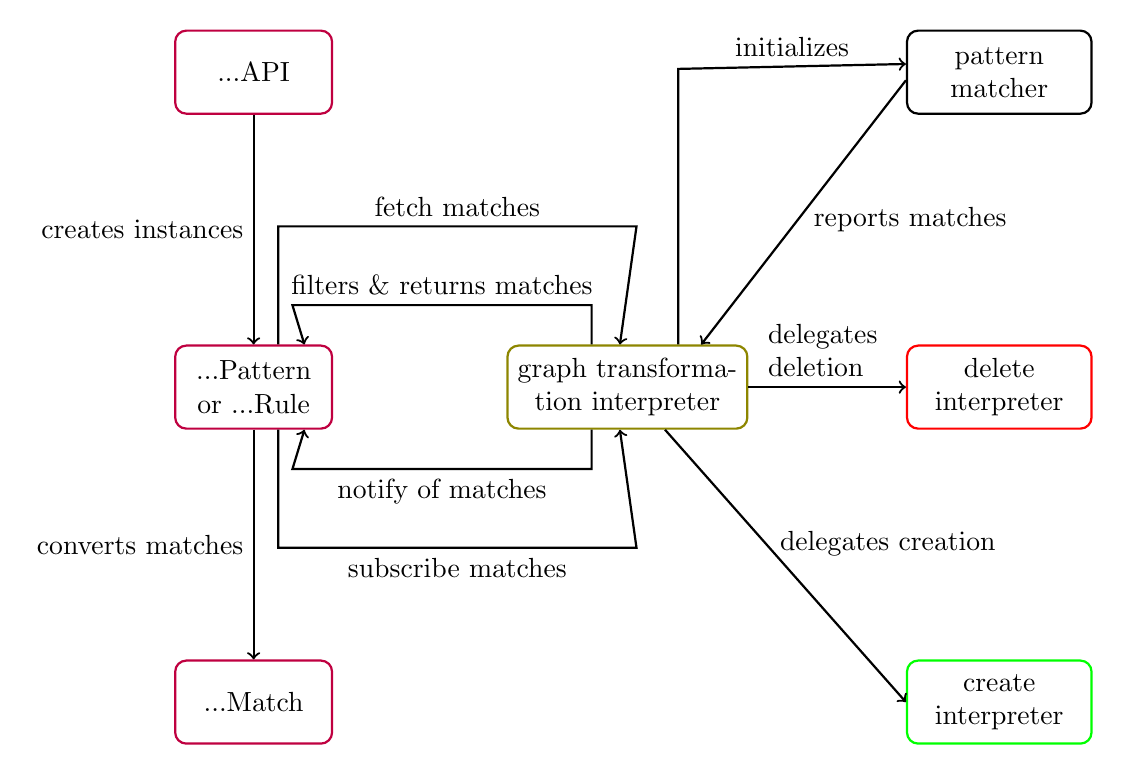
\begin{tikzpicture} [
		auto,
		node distance = 4cm,
		node/.style = {
			rectangle,
			rounded corners,
			thick,
			text width = 6em,
			text centered,
			minimum height = 3em
		},
		api/.style = {
			node,
			text width = 5em,
			draw = purple
		},
		gt-interpreter/.style = {
			node,
			text width = 8em,
			draw = olive
		},
		edge/.style = {
			->,
			thick
		}
	]

	\node[api] (api) {
		...API
	};
	\node[api, below of = api] (pattern) {
		...Pattern \\
		or ...Rule
	};
	\node[api, below of = pattern] (match) {
		...Match
	};

	\node[gt-interpreter, right = 2.2cm of pattern] (interpreter) {
		graph transformation interpreter
	};

	\node[node, draw = red, right = 2cm of interpreter] (delete-interpreter) {
		delete interpreter
	};
	\node[node, draw = black, above of = delete-interpreter] (context-interpreter) {
		pattern matcher
	};
	\node[node, draw = green, below of = delete-interpreter] (create-interpreter) {
		create interpreter
	};

	\draw[edge] (api) -- node[left] {creates instances} (pattern);
	\draw[edge] (pattern) -- node[left] {converts matches} (match);

	\draw[edge] (pattern.60) -- ++(0,1.5) -- ++(4.55,0) node[above, pos = 0.5] {fetch matches}  -- (interpreter.100);
	\draw[edge] (interpreter.130) -- ++(0,0.5) -- ++(-3.8,0) node[above, pos = 0.5] {filters \& returns matches} -- (pattern.40);
	
	\draw[edge] (pattern.300) -- ++(0,-1.5) -- ++(4.55,0) node[below, pos = 0.5] {subscribe matches} -- (interpreter.260);
	\draw[edge] (interpreter.230) -- ++(0,-0.5) -- ++(-3.8,0) node[below, pos = 0.5] {notify of matches} -- (pattern.320);
	
	\draw[edge] (interpreter.40) -- ++(0,3.5) -- node[] {initializes} (context-interpreter.175);
	\draw[edge] (context-interpreter.185) -- node[yshift = 0.2cm] {reports matches} (interpreter.30);
	\draw[edge] (interpreter) -- node[text width = 1.5cm] {delegates deletion} (delete-interpreter);
	\draw[edge] (interpreter) -- node[xshift = -0.2cm] {delegates creation} (create-interpreter.west);
\end{tikzpicture}

	\caption{API and Graph Transformation Interpreter}
	\label{fig:api-and-interpreter}
\end{figure}

\noindent
The graph transformation interpreter initializes the pattern matching engine (Democles) by registering the pattern set.
Democles will report any appearing and disappearing matches such that the graph transformation interpreter can maintain a set of \texttt{IMatch}es for each pattern.
\texttt{IMatch}es are an untyped representation of matches, which abstracts from the structure in the concrete pattern matching engine.

Remember that the API class is a factory for patterns and rules, \ie the methods return an instance of a pattern or a rule.
On a pattern/rule instance nodes and parameters can be bound to a fixed value (cp. the following section for details).
When a method for querying matches is called on a pattern or a rule, the call is delegated to the graph transformation interpreter which will return the matches as a \texttt{Stream} of \texttt{IMatch}es.
Using a \texttt{Stream}, unnecessary conversions between \texttt{Stream}s and collections can be avoided in the implementation of the API.
If nodes are bound or parameters are set, the matches will be filtered according to the fixed nodes or parameter values.
If a pattern is defined as being one of multiple alternative patterns, the graph transformation interpreter will combine the matches of all alternative patterns and remove duplicates (cp. Section~\ref{disjunctions}).
Before a pattern or a rule returns the matches, these matches are converted to a typed representation.

Before a rule can be applied, a match must be found where the rule can be applied to.
If a rule contains only created elements, the rule is always applicable. An empty match will be generated in this special case.
Rule applications are delegated to the delete and the create interpreter which handle the rule application according to the defined pushout approach using the create or delete patterns from the IBeX model.

\section{Usage of the API}
\label{api-usage}
This section deals with the usage of the Java API.
The API features are explained using small example code snippets.

\subsection{Initialization and Conventions on EMF Resources}
\label{api-conventions}
An EMF model is assumed to be represented by a \texttt{ResourceSet}, containing one or more resources (files, usually having the file extension \texttt{xmi}).
If not explicitly specified, the first resource in the \texttt{ResourceSet} is chosen as default resource.
All created nodes whose resource is not determined automatically due to their container object, will be placed in the default resource.
Deleted nodes will be moved to a trash resource, which is created automatically.

The generated app class provides convenient methods for model initialization and setting the default resource.
The meta-models used by the patterns and rules in the API will be registered automatically.
The easiest way to initialize an API with a model is to implement a subclass of the Democles app generated in the API package, as shown in Listing~\ref{listing:loading-models}.
As the method names suggest, the method \texttt{createModel(URI)} creates a new empty resource with the given URI, while \texttt{loadModel(URI)} loads an existing resource.

In this case, the file \texttt{newModel.xmi} will be the default resource such that created elements will be added to this file -- except if the container of the created elements is an object in the file \texttt{model.xmi}.
To use \texttt{model.xmi} as the default resource, it can be set via \texttt{setDefaultResource(Resource)}. Alternatively, changing the order of the two method calls adding a resource to the model will lead to the same result.

\begin{lstlisting}[caption={Loading Models}, label={listing:loading-models}]
public class MyGTApp extends SheRememberedCaterpillarsGraphTransformationDemoclesApp {
	SheRememberedCaterpillarsGraphTransformationAPI api;

	public MyGTApp() {
		String path = "./instances/";
		createModel(URI.createFileURI(path + "newModel.xmi"));
		loadModel(URI.createFileURI(path + "model.xmi"));

		api = initAPI();
	}

	public static void main(String[] args) {
		new MyGTApp();
	}
}
\end{lstlisting}

\subsection{Model Queries}
\label{api-model-queries}
Listing~\ref{listing:model-queries} shows examples how the model can be queried via the API using the pattern \texttt{findCharacterOnExit} (Figure~\ref{fig:pattern-findCharacterOnExit}).
All methods for querying matches fetch the untyped matches from the interpreter and convert the matches into the typed representation.
To get the number of matches, one should always use the method \texttt{countMatches()} because the implementation avoids the conversion.

\begin{lstlisting}[caption={Model Queries}, label={listing:model-queries}]
public Optional<Character> findAnyCharacter() {
	return api.findCharacterOnExit()
		.findAnyMatch()
		.map(m -> m.getCharacter());
}

public List<Character> findAllCharacters() {
	return api.findCharacterOnExit()
		.matchStream()
		.map(m -> m.getCharacter())
		.collect(Collectors.toList());
}

public long countCharacters() {
	return api.findCharacterOnExit().countMatches();
}
\end{lstlisting}

\subsection{Rule Applications and Pushout Approaches (DPO vs. SPO)}
\label{api-pushout-approaches}
Rules can be applied via the \texttt{apply()} method, which returns an \texttt{Optional} for the co-match.
The \texttt{Optional} may be empty if the rule is not applicable.\footnote{A rule is not applicable if there is no match for the rule or the DPO approach forbids the rule application on the chosen match due to dangling edges.}
Per default rules are applied according to the single pushout approach such that any dangling edges are deleted.
This behavior can be changed on API level (holds for all future rule applications which do not overwrite this setting), for all applications of a certain rule or for a concrete rule application.

In Listing~\ref{listing:dpo} the rule is applied via DPO.
Note that the set pushout approach holds just for this rule.
To enable DPO for the applications of all rules, the setting must be changed on API level via \texttt{api.setDPO()}.

\begin{lstlisting}[caption={Usage of DPO for a Single Rule Application}, label={listing:dpo}]
public void moveDPO() {
	api.moveCharacterToNeighboringPlatform()
		.setDPO()
		.apply()
		.ifPresent(m -> {
			String name = m.getCharacter().getName();
			System.out.println("Character " + name + " moved to neighboring platform");
		});
}
\end{lstlisting}

\subsection{Node Bindings}
\label{api-node-bindings}
By default all nodes of a pattern are unbound, \ie they can be matched to any object of the correct type.
A node binding fixes a node to a specific object.
At runtime the graph transformation interpreter filters the matches reported by the pattern matching engine for those whose nodes are bound to the same objects as defined by the node binding.

A node binding can be defined for all context nodes and deleted nodes (except local nodes).\footnote{Since local nodes are not contained in matches, so local nodes cannot be used as a filter on matches.}
The API provides typed \texttt{bind} methods for those nodes.
For convenience there are methods to bind all parameters of any match to the nodes of the same name.
This allows to pass the bound objects in a match result of a model query or a rule application directly to another query or rule.

Listing~\ref{listing:node-binding} gives an example for the usage of node bindings:
The query selects an arbitrary character which is not on an exit platform.
After that, this character is bound to the application of the rule \texttt{moveCharacterToNeighboringPlatform} (Figure~\ref{fig:rule-moveCharacterToNeighboringPlatform}) such that only the selected character can be moved if a match for the rule can be found.
The method \texttt{moveCharacter2} in Listing~\ref{listing:node-binding2} does exactly the same as \texttt{moveCharacter}, since \texttt{character} is the only node name which occurs both in the pattern \texttt{findCharacterNotOnExit} and in the rule \texttt{moveCharacterAcrossBridge} (cp. Figure~\ref{fig:node-binding-common-nodes}).
So the \texttt{bind}-method will bind only the character and ignore the other nodes.

\begin{lstlisting}[caption={Node Binding}, label={listing:node-binding}]
public void moveCharacter() {
	api.findCharacterNotOnExit()
		.findAnyMatch()
		.ifPresent(m -> {
			api.moveCharacterToNeighboringPlatform()
				.bindCharacter(m.getCharacter())
				.apply();
		});
}
\end{lstlisting}

\begin{lstlisting}[caption={Node Binding based on Naming Convention}, label={listing:node-binding2}]
public void moveCharacter2() {
	api.findCharacterNotOnExit()
		.findAnyMatch()
		.ifPresent(m -> {
			api.moveCharacterToNeighboringPlatform()
				.bind(m)
				.apply();
		});
}
\end{lstlisting}

\begin{figure}[h!]
	\centering
	\includegraphics[scale=0.7]{../common/figures/pattern-findCharacterNotOnExit}
	\includegraphics[scale=0.7]{../common/figures/rule-moveCharacterToNeighboringPlatform}
	\caption{Common Nodes of the Pattern \texttt{findCharacterNotOnExit} and the Rule \texttt{moveCharacterToNeighboringPlatform}}
	\label{fig:node-binding-common-nodes}
\end{figure}

\subsection{Parameters}
\label{api-parameters}
Patterns and rules may define parameters of primitive data types to be used in attribute assignments or conditions.
In contrast to node bindings, parameters are required.
When calling a pattern or rule, all parameters must be set in the constructor.
The parameter values may be changed using the setters.

Attribute conditions with parameters are filtered by the graph transformation interpreter similar to node bindings while all  other attribute conditions are checked by the pattern matching engine.
Parameterized attribute assignments will set the value of the parameter as new attribute value.
An example for this is shown in Listing~\ref{listing:parameters}:
The parameter for the color is passed to the pattern \texttt{findCharacterOfColor} (Figure~\ref{fig:pattern-findCharacterOfColor}) in the constructor (so it cannot be omitted!).
Without the parameter, the attribute condition could not be evaluated.
The interpreter knows all matches for the pattern reported by Democles and filters those for the ones whose color attribute has the given value \texttt{BLUE}.

\begin{lstlisting}[caption={Parameters}, label={listing:parameters}]
public void outputBlueCharacters() {
	api.findCharacterOfColor(COLOR.BLUE)
		.forEachMatch(m -> {
			System.out.println(m.getCharacter().getName());
		});
}
\end{lstlisting}

\section{Exploiting the Incrementality}
\label{incrementality}
As eMoflon::IBeX-GT is based on an incremental pattern matcher, the incrementality can be exploited to support certain scenarios which are more difficult to implement without support for incrementality.
The following sections describe tasks which could not be easily supported without incrementality because they require permanent observation of all matches.
The incremental features add support for reactive programming \cite{SurveyReactiveProgramming}, which is based on automatic propagation of changes.

\subsection{Notification System}
\label{notification-system}
The pattern matcher permanently maintains a set of matches for all patterns and notifies the interpreter every time a new match appears or an existing match disappears.
This can be used to provide a notification system in the API: Subscribers can register themselves for notifications of appearing and disappearing matches.
If subscribers are registered, the interpreter forwards the notification of appearing or disappearing matches to them.

One application scenario is the permanent checking of constraints via reception of notifications whenever matches for the observed pattern appear or disappear.
For positive constraints there must be a match, otherwise the constraint is violated.
For negative constraints any reported match is a violation of the constraint.

In the context of the She Remembered Caterpillars game the notification system could be used to check whether the goal of the game (all characters stand on an exit platform) is reached by subscribing all matches for a character not on an exit platform:
As soon as the number of characters which are not on an exit platform reaches 0, the game is over.
Note that one needs to subscribe to the disappearing matches as well such that characters leaving an exit platform are added to the set again.
Listing~\ref{listing:notifications} shows the necessary code for initializing and maintaining the set of characters which have not reached their final destination yet.
The defined \texttt{Consumer}s will be called automatically whenever a change in the set of matches for the subscribed pattern is reported.

Without the notification system, one would need to check the subscribed pattern after every change in the model to be sure to notice that the game is over as soon as the last character reached an exit platform.
The incremental pattern matcher notices even changes made by third party-applications and not via the API -- and the changes in the set of matches triggers notifications if a subscription has been registered for those.

\begin{lstlisting}[caption={Subscription of Notifications}, label={listing:notifications}]
Set<Character> characters = new HashSet<Character>();

public void registerSubscriptions() {
	FindCharacterNotOnExitPattern notOnExit = api.findCharacterNotOnExit();
	notOnExit.matchStream()
		.map(m -> m.getCharacter())
		.forEach(c -> this.characters.add(c));
	notOnExit.subscribeDisappearing(m -> {
		this.characters.remove(m.getCharacter());
		checkEndOfGame();
	});
	notOnExit.subscribeAppearing(m -> {
		this.characters.add(m.getCharacter());
		checkEndOfGame();
	});
}

private void checkEndOfGame() {
	if (this.characters.size() == 0) {
		System.out.println("GAME OVER!");
	}
}
\end{lstlisting}

\subsection{Instant Automatic Rule Application}
\label{instant-automatic-rule-application}
Due to the notification of appearing matches, instant and automatic rule application can be easily supported.
If automatic rule application is enabled, the notification system will send a notification and the interpreter will apply the rule immediately after the new match appeared.
Note that this only holds for matches reported after enabling automatic rule applications.
Rule applications can be subscribed via the API's notification system.

Listing~\ref{listing:instant-application} shows an example of enabling automatic rule application.
Assuming that the rule \texttt{transformBlueAndRedToPurpleCharacter} (Figure~\ref{fig:rule-transformBlueAndRedToPurpleCharacter}) shall be applied as soon as a match for this rule is found, \ie a blue and a red character stand on the same platform.
Via a subscription of the rule applications, a \texttt{Consumer} outputs ``Automatic transformation'' on the console whenever the rule is applied.

\begin{lstlisting}[caption={Instant Automatic Rule Application}, label={listing:instant-application}]
public void enableAutoTransformations() {
	TransformBlueAndRedToPurpleCharacterRule transformation = api.transformBlueAndRedToPurpleCharacter();
	transformation.subscribeRuleApplications(m -> 
		System.out.println("Automatic transformation"));
	transformation.enableAutoApply();
}
\end{lstlisting}

\begin{figure}[h!]
	\centering
	\includegraphics[scale=0.7]{../common/figures/rule-transformBlueAndRedToPurpleCharacter}
	\caption{Rule \texttt{transformBlueAndRedToPurpleCharacter}}
	\label{fig:rule-transformBlueAndRedToPurpleCharacter}
\end{figure}

	% !TeX encoding = UTF-8
% !TeX spellcheck = en_US

\section{Evaluation and Future Work}
	\begin{frame}
		\frametitle{Contents}
		\tableofcontents[currentsection]
	\end{frame}
	\begin{frame}
		\frametitle{Evaluation and Future Work}
		\framesubtitle{Compliance with Requirements, JUnit Tests}
		\begin{itemize}
			\item Requirements fulfilled
				\begin{itemize}
					\item Application conditions only in DNF
					\item Limited set of attribute assignments and conditions
				\end{itemize}

			\only<2-3>{
			\item 2 JUnit test suites for 13 APIs with 90 test cases
				\begin{itemize}
					\item TestsuiteGT covers 90\,\% of the abstract classes and the interpreter
					\item Build of GT projects covers 94\,\% of the GT builder
					\item used in MBSE lecture (Summer Term 2018)
				\end{itemize}
			\item JUnit test suite for scoping/validation in the editor: 111 test cases, coverage 96\,\%
			}
		\end{itemize}
	\end{frame}
	\begin{frame}
		\frametitle{Evaluation and Future Work}
		\framesubtitle{End-User Survey: Textual Syntax and Visualization}
		\begin{center}
			\includegraphics[width=\linewidth]{../common/figures/evaluation-results-syntax}
		\end{center}
	\end{frame}
	\begin{frame}
		\frametitle{Evaluation and Future Work}
		\framesubtitle{End-User Survey: Java Integration}
		\begin{center}
			\includegraphics[width=.7\linewidth]{../common/figures/evaluation-results-java-integration}
		\end{center}
	\end{frame}
	\begin{frame}
		\frametitle{Evaluation and Future Work}
		\framesubtitle{Performance of Model Generation and Modification (linear time axis)}
		\begin{center}
			\includegraphics[height=.75\textheight]{../common/figures/evaluation-runtime1}
		\end{center}
	\end{frame}
	\begin{frame}
		\frametitle{Evaluation and Future Work}
		\framesubtitle{Performance of Model Generation and Modification (logarithmic time axis)}
		\begin{center}
			\includegraphics[height=.75\textheight]{../common/figures/evaluation-runtime1-logarithmic}
		\end{center}
	\end{frame}
	\begin{frame}
		\frametitle{Evaluation and Future Work}
		\framesubtitle{Performance of Model Queries (linear time axis)}
		\begin{center}
			\includegraphics[height=.75\textheight]{../common/figures/evaluation-runtime2}
		\end{center}
	\end{frame}
	\begin{frame}
		\frametitle{Evaluation and Future Work}
		\framesubtitle{Performance of Model Queries (logarithmic time axis)}
		\begin{center}
			\includegraphics[height=.75\textheight]{../common/figures/evaluation-runtime2-logarithmic}
		\end{center}
	\end{frame}
	\begin{frame}
		\frametitle{Evaluation and Future Work}
		\framesubtitle{Summary and Future Work}
		\begin{block}{eMoflon::IBeX-GT}
			\begin{itemize}
				\item Expressive pattern language with simple syntax
				\item Integration into Java via a generated, typed API
				\item Incremental features
				\item Shared libraries with eMoflon::IBeX-TGG
			\end{itemize}
		\end{block}

		\only<2>{
		\begin{block}{Future work}
			\begin{itemize}
				\item Evaluation of performance
				\item Optimization of the pattern network
				\item Shared IBeX patterns with TGG
			\end{itemize}
		\end{block}
		}
	\end{frame}

	% !TeX encoding = UTF-8
% !TeX spellcheck = en_US

\chapter{Conclusion and Future Work}
\label{future-work}
This thesis presented eMoflon::IBeX-GT, a new graph transformation tool with a Java API exploiting the incrementality of its underlying pattern matching engine, Democles.
It provides mature support for all requirements from Chapter~\ref{requirements} with some minor restrictions (cp. Sections~\ref{evaluation-requirements} and~\ref{expressiveness}).
In Chapter~\ref{related-work} we have seen that no other GT tool supports all requirements.

\section{Evaluation of Performance}
\label{evaluation-of-performance}
As performance is not the focus of this work, performance has only been evaluated shortly with respect to scalability for models of different sizes.
The evaluation in Section~\ref{evaluation-performance} clearly indicates that the maximal model size which can be handled by eMoflon::IBeX is limited by the available main memory.
It also shows that the time for creation is linear to the number of created elements, but the time for answering queries on the model is nearly constant.
The incrementality helps to reach a constant response time for model queries, as the matches are not searched on demand, but maintained permanently.
However, queries with bound parameters seem to have a worse performance as filtering the matches reported by Democles is necessary.

\section{Optimization of the Pattern Network}
\label{pattern-optimization}
Due to a missing detailed evaluation of the performance, optimizing the pattern network generated for the graph transformation specification with respect to performance remains as future work.
The insights for optimizing the patterns of eMoflon::IBeX-TGG by Weidmann (see \cite{ConsistencyManagementViaCombinationOfTGGAndILP}, Section 5.2) could be a useful starting point for the optimization.
eMoflon::IBeX-TGG has configuration flags for the different possible patterns (\eg whether all edges are extracted into an invoked pattern) such that the user can evaluate which configuration is best for the used TGG rules.
A similar approach could be implemented for GT, hopefully improving the performance for many pattern specifications.

Currently the transformation from the editor model into the IBeX model does not exploit the refinement hierarchy.
Instead the patterns are flattened into a structure without refinement before the transformation.
It could be checked whether the refinement hierarchy can be exploited for the pattern network to improve the performance.
However, a similar approach for the TGG part \cite{ExploitingTheModularityOfTGGs} has not shown significant performance improvements.

\section{Shared Patterns with eMoflon::IBeX-TGG}
\label{shared-patterns}
In future, IBeX patterns should be shared with the TGG part of eMoflon::IBeX.
The IBeX pattern model is designed such that this should be easily possible.
Just for attributes the IBeX model cannot handle the complexity of attribute constraints necessary for eMoflon::IBeX-TGG such that a little extension of the IBeX model is required.
Technically, the following steps are necessary to use the IBeX pattern model in the TGG part as well:
\begin{itemize}
	\item the extension of the IBeX pattern meta-model such that attribute constraints can be specified in the complexity necessary for TGG specifications (especially user-defined attribute constraints),
	\item the transformation of the internal TGG model to the IBeX pattern model,\footnote{Alternatively a direct transformation from the editor TGG model to the IBeX pattern model could be implemented, but this would be a huge step, as the IBeX pattern model completely abstracts from TGGs.}
	\item the adaption of the transformation from the IBeX pattern model to Democles patterns (and the initialization of the Democles patterns in the \texttt{DemoclesGTEngine}) to handle the additional attribute constraints (after that the transformation from \texttt{IBlackPattern}s to Democles patterns in the TGG part can be removed),
	\item the removal of the pattern initialization in the \texttt{DemoclesTGGEngine} (because this can be inherited from the \texttt{DemoclesGTEngine} as soon as both engines are initialized with IBeX patterns),
	\item and the adaptation of the green and red interpreter for TGGs (handling creation and deletion during rule applications), their interfaces, and the operational strategies using them.
\end{itemize}

\noindent
Maybe the current \texttt{IbexGreenInterpreter} for TGGs can be even replaced with the \texttt{GraphTransformationCreateInterpreter}, if create patterns are generated in the IBeX pattern model.
For the red interpreter an own implementation for the TGG part will remain necessary, as deletion for TGGs is undoing a previous rule application instead of applying the deletions specified by a delete pattern.

\section{Applications using Graph Transformation and TGG}
\label{applications-using-gt-and-tggs}
Besides the integration of eMoflon::IBeX-GT and eMoflon::IBeX-TGG from the perspective of the eMoflon::IBeX development team, both parts can also be used together by end-users.
An example is the usage of graph transformation for preprocessing a model synchronized with another model via a TGG.\footnote{The eMoflon::IBeX-TGG handbook \cite{eMoflonIBeX-TGG-Handbook} provides an example for GT as a preprocessor.}
Currently this is possible, but requires some knowledge how the pattern matcher works.

After eMoflon::IBeX has been migrated to the IBeX pattern model, it may be possible to use only one Democles engine instance in an application using a GT API and a TGG in order to save memory and sharing common patterns (\eg edge patterns).
Currently the GT API and the operationalization for the TGG use two different engines.

\section{Expressiveness of the Graph Transformation Rules}
\label{expressiveness}
The specification of attribute assignments and conditions is currently restricted to a subset of the theoretical possibilities.
Regarding attributes, the reason is a lack of time during the implementation of this thesis.
In the future it could be evaluated whether the implemented subset is satisfying for all use cases.
However, the API allows to set arbitrary attribute values after rule applications (\eg via a subscription of rule applications with a \texttt{Consumer} calculating and setting the attribute value in self-written Java code).
After eMoflon::IBeX-TGG has been refactored to use IBeX patterns as well, the IBeX model needs to support more complex attribute conditions.
So just the editor and the transformation from editor patterns to IBeX patterns has to be extended.

The support for complex graph conditions is restricted to expressions in DNF, which does not limit the expressiveness.
In general, this can lead to longer logical expressions the user has to define.
Technical limitations of the currently used pattern matching engine are the reason for this decision, as Democles cannot handle alternatives.
As described in Section~\ref{disjunctions}, the matches for the alternatives are collected separately and merged by the interpreter.
This approach ensures that as much as possible of the work is done by the pattern matcher, which ensures that invalid matches are filtered out in the first step already.
In the case that support for alternatives is implemented in Democles, the implementation could be adjusted to check the alternatives directly in Democles which avoids combining and removing duplicates in the graph transformation interpreter.

If it turns out that the restriction to expressions in DNF is disturbing of many users, one could allow arbitrary logical expressions in the editor and transform the expression into the DNF before the patterns are transformed.

\section{Improvements to the Editor}
\label{improvements-to-the-editor}
The feedback of end-users pointed out that a link between editor patterns/rules and Java classes would be helpful (cp. Section~\ref{evaluation-java-integration}).
A visualization is intentionally not editable according to our requirements list, as this requires a more complex implementation and the handling of the layout.
Although some end-users have suggested an editable visual syntax, our initial consideration has not changed.

Currently the syntax for the textual specification in the GT and TGG editor and the formatting algorithms are not completely consistent.
This should be adjusted for full consistency between GT and TGG.



% Appendix
	\appendix

% Lists
	% !TeX encoding = UTF-8
% !TeX spellcheck = en_US
\chapter{List of Projects}
\label{appendix-list-of-projects}

\begin{figure}[h!]
	\centering
	% !TeX encoding = UTF-8
% !TeX spellcheck = en_US

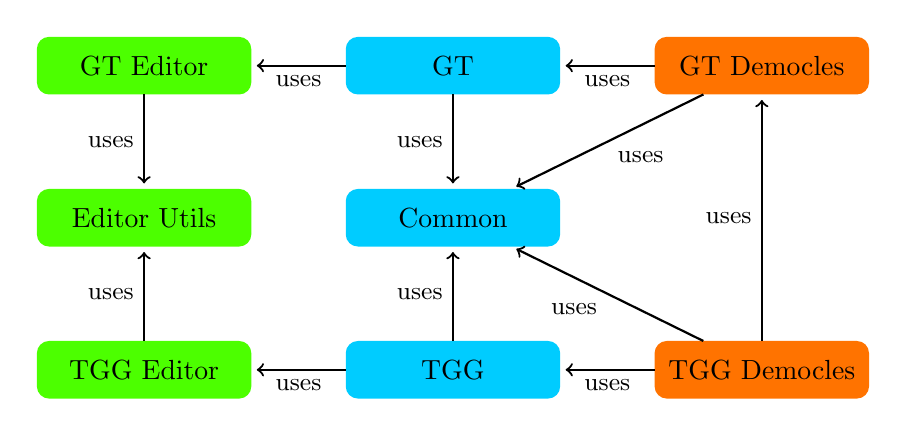
\begin{tikzpicture} [
		auto,
		node/.style = {
			rectangle,
			rounded corners,
			thick,
			text width = 7em,
			text centered,
			minimum height = 2em,
		},
		line/.style = {
			draw,
			thick,
			->,
			shorten >=2pt,
		},
		line-caption/.style = {
			font = \small,
		},
		ibex-ui/.style = {
			draw = green!60!lime,
			fill = green!60!lime,
		},
		ibex/.style = {
			draw = blue!20!cyan,
			fill = blue!20!cyan,
		},
		ibex-democles/.style = {
			draw = red!10!orange,
			fill = red!10!orange
		}
	]

	\matrix[
		column sep = 12mm,
		row sep = 12mm
	] {
		\node[node, ibex-ui] (uiGT) {
			GT Editor
		};
		& \node[node, ibex](GT) {
			GT
		};
		& \node[node, ibex-democles](democlesGT) {
			GT Democles
		};
		\\
		\node[node, ibex-ui] (uiCommon) {
			Editor Utils
		};
		& \node[node, ibex](common) {
			Common
		};
		\\
		\node[node, ibex-ui] (uiTGG) {
			TGG Editor
		};
		& \node[node, ibex](TGG) {
			TGG
		};
		& \node[node, ibex-democles](democlesTGG) {
			TGG Democles
		};
		\\
	};

	\begin{scope} [
		every path/.style = line,
		every node/.style = line-caption
		]
		\path (uiGT) -- node[left] {uses} (uiCommon);
		\path (uiTGG) -- node[left] {uses} (uiCommon);

		\path (GT) -- node {uses} (uiGT);
		\path (TGG) -- node {uses} (uiTGG);

		\path (GT) -- node[left] {uses} (common);
		\path (TGG) -- node[left] {uses} (common);

		\path (democlesGT) -- node {uses} (GT);
		\path (democlesGT) -- node {uses} (common);
		\path (democlesTGG) -- node {uses} (common);
		\path (democlesTGG) -- node {uses} (TGG);
		\path (democlesTGG) -- node {uses} (democlesGT);
	\end{scope}
\end{tikzpicture}
 \\
	(cp. Section~\ref{emoflon-ibex-architecture})
\end{figure}

\begin{longtable}[h!]{lll}
	\toprule
	Repository
		& Component
		& Plugin Project \\
	\midrule
	emoflon-ibex-ui\footnote{\url{https://github.com/eMoflon/emoflon-ibex-ui}}
		& Editor Utils
		& \texttt{org.emoflon.ibex.editor.utils} \\		
		& GT Editor
		& \vtop{
			\hbox{\texttt{org.emoflon.ibex.gt.editor}}
			\hbox{\texttt{org.emoflon.ibex.gt.editor.ide}}
			\hbox{\texttt{org.emoflon.ibex.gt.editor.ui}}
		} \\
		& TGG Editor
		& \vtop{
			\hbox{\texttt{org.emoflon.ibex.tgg.editor}}
			\hbox{\texttt{org.emoflon.ibex.tgg.editor.ui}}
			\hbox{\texttt{org.emoflon.ibex.tgg.ide}}
		} \\
	\midrule
	emoflon-ibex\footnote{\url{https://github.com/eMoflon/emoflon-ibex}}
		& Common
		& \texttt{org.emoflon.ibex.common} \\
		& GT
		& \texttt{org.emoflon.ibex.gt} \\
		& TGG
		& \vtop{
			\hbox{\texttt{org.emoflon.ibex.core.language}}
			\hbox{\texttt{org.emoflon.ibex.core.runtime}}
		} \\
	\midrule
	emoflon-ibex-democles\footnote{\url{https://github.com/eMoflon/emoflon-ibex-democles}} 
		& GT Democles
		& \texttt{org.emoflon.ibex.gt.democles} \\
		& TGG Democles
		& \vtop{
			\hbox{\texttt{org.emoflon.ibex.tgg.ide.democles}}
			\hbox{\texttt{org.emoflon.ibex.tgg.runtime.democles}}
		} \\
	\bottomrule
	\caption{List of Projects in the eMoflon::IBeX Tool Suite}
\end{longtable}

	\listoffigures
	\listoftables
	\lstlistoflistings

% Bibliography
	\bibliography{../common/literature}
	\bibliographystyle{alpha}
	\label{bibliography}	
\end{document}
